\documentclass[12pt]{report}

%\usepackage[a4paper, left = 2.5cm, top = 2.5cm, bottom = 2cm, right = 2cm]{geometry}
%\usepackage{showframe}
\usepackage{vmargin}

\setpapersize{A4}
\setmargins{3cm}       % margen izquierdo
{2.5cm}                  % margen superior
{15.5cm}                 % anchura del texto
{23.7cm}                % altura del texto
{0pt}                   % altura de los encabezados
{0cm}                    % espacio entre el texto y los encabezados
{10pt}                    % altura del pie de página
{1cm}                    % espacio entre el texto y el pie de página



\usepackage[spanish,es-tabla]{babel} % Idioma español con tablas
\usepackage{longtable}     % Usado para diseñar grandes tablas.
\usepackage{multirow} % para las tablas

\usepackage{amsmath, amssymb, amsfonts, latexsym, anyfontsize}
\usepackage{color, alltt, times}
\setcounter{secnumdepth}{3} %para que ponga 1.1.1.1 en subsubsecciones
\setcounter{tocdepth}{3}    % para que ponga subsubsecciones en el indice
\usepackage{setspace}       % Usado para %\onehalfspace  \doublespacing  \singlespace
\usepackage{booktabs}       % Para formar tablas
\usepackage{appendix}       % para los anexos
\usepackage{url}            % para citar las urls
\usepackage{pdfpages}       % para insertar documentos de tipo PDF en latex
\usepackage{epstopdf}       % para insertar imagenes en formato eps obtenidas en Matlab
\usepackage{graphicx}       % para las imagenes y gráficos
\usepackage{subfigure}      % para subfiguras
%\usepackage[round]{natbib}
\usepackage[utf8]{inputenc}         % Para escribir en castellano
\usepackage[T1]{fontenc}

\usepackage{algorithmic}
\usepackage{algorithm}
\floatname{algorithm}{Algoritmo}
\renewcommand{\listalgorithmname}{Lista de algoritmos}
\renewcommand{\algorithmicrequire}{\textbf{Entrada:}}
\renewcommand{\algorithmicensure}{\textbf{Salida:}}
\renewcommand{\algorithmicend}{\textbf{FIN}}
\renewcommand{\algorithmicif}{\textbf{SI}}
\renewcommand{\algorithmicthen}{\textbf{ENTONCES}}
\renewcommand{\algorithmicelse}{\textbf{CASO CONTRARIO}}
\renewcommand{\algorithmicelsif}{\algorithmicelse,\ \algorithmicif}
\renewcommand{\algorithmicendif}{\algorithmicend\ \algorithmicif}
\renewcommand{\algorithmicfor}{\textbf{PARA}}
\renewcommand{\algorithmicforall}{\textbf{para todo}}
\renewcommand{\algorithmicdo}{\textbf{HACER}}
\renewcommand{\algorithmicendfor}{\algorithmicend\ \algorithmicfor}
\renewcommand{\algorithmicwhile}{\textbf{MIENTRAS}}
\renewcommand{\algorithmicendwhile}{\algorithmicend\ \algorithmicwhile}
\renewcommand{\algorithmicloop}{\textbf{REPETIR}}
\renewcommand{\algorithmicendloop}{\algorithmicend\ \algorithmicloop}
\renewcommand{\algorithmicrepeat}{\textbf{REPETIR}}
\renewcommand{\algorithmicuntil}{\textbf{HASTA}}
\renewcommand{\algorithmicprint}{\textbf{imprimir}} 
\renewcommand{\algorithmicreturn}{\textbf{RETORNAR}} 
\renewcommand{\algorithmictrue}{\textbf{cierto }} 
\renewcommand{\algorithmicfalse}{\textbf{falso }} 
 % mi archivo de traducción

\usepackage[x11names,table]{xcolor}

\usepackage{tikz,tkz-tab, tcolorbox}
\usepackage{caption}
\usepackage[round]{natbib} 
\usepackage{listings}
 
\begin{document}


\baselineskip 1cm
\pagestyle{plain}
%%%%%%%%%%%%%%%%%%%%%%%%%%%%% CARATULA%%%%%%%%%%%%%%%%%%%%%%%%
\textheight 19cm
\pagestyle{empty}
\begin{center}
 {\bf {\fontsize{14}{16.8}\selectfont UNIVERSIDAD NACIONAL DE TRUJILLO}}     
 
    {\bf{\fontsize{14}{16.8}\selectfont Facultad de Ciencias Físicas y Matemáticas}} 

  {\bf{\fontsize{14}{16.8}\selectfont Escuela Profesional de Informática}}
\end{center}  

\begin{figure}[ht]
\begin{center}

\includegraphics[width=.4\textwidth]{unt}
\end{center}
\end{figure}
\vskip 0.5cm

\begin{center}
  {\bf\Large{{\fontsize{17}{20.4}\selectfont{Sistema Basado en Conocimiento Mediante RNA para Pronósticar las Ventas en el Mall Aventura} }}}     
\end{center}
\vskip 0.5cm

\begin{center}
{\Large{TESIS}}
\end{center}
\begin{center}
{\large{\hspace*{0.4cm} PARA OPTAR EL TÍTULO PROFESIONAL DE INGENIERO  INFORMÁTICO}}
\end{center}

\vskip 0.6cm
\begin{center}
  { \fontsize{14}{16.8}\selectfont {\hspace{-2.9cm}AUTOR:  \ Lopez Andrade Alex Michael Andre   }} \\
    \vskip 0.2cm
    { \fontsize{14}{16.8}\selectfont {\hspace{-1.7cm} ASESOR: Mg. Bravo Escalante Jorge David  }}

     
\end{center}   


\vskip 1.1cm
\begin{center}    
{\bf {\fontsize{14}{16.8}\selectfont TRUJILLO - PERÚ
\vskip 0.0cm
\hspace*{-0.2cm} 
2020 }}
\end{center} 
\newpage
%%%%%%%%%%%%%%%%%%%%%%%%%%%%%%%%%%%%%%%%%%%%%%%%%%%%%%%%%%%%%%%%%%%%%%%%%%%


%%%%%%%%%%%%%%%%%%%%%%%%%%%%CONTRA CARATULA 1 %%%%%%%%%%%%%%%%%%%%%%%%%%%%%
%\newpage
\pagestyle{plain}
\pagenumbering{roman}
%
\hspace*{6cm}
\vskip 9cm
\begin{center}
%   {\bf \doublespacing {\fontsize{17}{20.4}\selectfont{SISTEMA BASADO EN CONOCIMIENTO MEDIANTE RNA PARA PRONÓSTICAR LAS VENTAS EN EL MALL AVENTURA }}}     
\end{center} 
\newpage
%%%%%%%%%%%%%%%%%%%%%%%%%%%%%%%%%%%%%%%%%%%%%%%%%%%%%%%%%%%%%%%%%%%%%%%%%%%
%
%
%%%%%%%%%%%%%%%%%%%%%%%%%%%%%% CONTRA CARATULA 2 %%%%%%%%%%%%%%%%%%%%%%%
\begin{center}
   {\bf {\fontsize{14}{16.8}\selectfont{PAUL DENIS SANCHEZ RODRIGUEZ}}}   
\end{center}   

\vskip 3.2cm
\begin{center}
   {\bf \doublespacing {\fontsize{17}{20.4}\selectfont{SISTEMA BASADO EN CONOCIMIENTO MEDIANTE RNA PARA PRONÓSTICAR LAS VENTAS EN EL MALL AVENTURA }}}     
\end{center}   
  \vskip 2cm
\begin{verse}
 \fontsize{12}{14.4}\selectfont{\hspace*{0.6cm}Tesis presentada a la Escuela Profesional de Informática en la Facultad de Ciencias Físicas y Matemáticas de la Universidad Nacional de Trujillo, como requisito parcial para la obtención del grado de Título profesional de Ingeniero Informático}
\end{verse}
%
\vskip 1.5cm 
{\fontsize{14}{16.8}\selectfont ASESOR: Mg. BRAVO ESCALANTE JORGE DAVID} 
 \vskip 1cm 
 \begin{center}    
 \vskip 2cm
{\fontsize{14}{16.8}\selectfont Trujillo - Perú
\vskip 0.2cm
\hspace*{-0.2cm} 
2020}
\end{center} 
\newpage
%%%%%%%%%%%%%%%%%%%%%%%%%%%%%%%%%%%%%%%%%%%%%%%%%%%%%%%%%%%%%%%%%%%%
%
%%%%%%%%%%%%%%%%%%%%%%%%%%%%%HOJA DE APROBACION %%%%%%%%%%%%%%%%%%%%%%%%%%%%%
\begin{center}
 {\bf {\Large HOJA DE APROBACIÓN }     
 \vskip 1.5cm
  {\Large Sistema Basado en Conocimiento Mediante RNA para Pronósticar las Ventas en el Mall Aventura }}
 \vskip 1cm 
  {\large{Paul Denis Sanchez Rodriguez}
 \vskip 1cm
\end{center} 
Tesis defendida y aprobada por el jurado examinador:
\vskip 1 cm
\begin{flushleft} 
$\overline{\mbox{Prof. Mg. Yenny M. Sifuentes Díaz - Asesor}}$\\
\vskip -0.5cm
Departamento de Informática - UNT
\end{flushleft} 
\vskip 1cm
\begin{flushleft} 
$\overline{\mbox{Prof. Mg. Ricardo Manuel Guevara Ruiz}}$\\
\vskip -0.5cm
Departamento de Informática - UNT
\end{flushleft} 
\vskip 1cm
\begin{flushleft} 
$\overline{\mbox{Prof. Mg. Sofía Pedro Huamán}}$\\
\vskip -0.5cm
Departamento de Informática - UNT
\end{flushleft}
\vskip 0.8cm 
\begin{center}    
Trujillo, 2020
\end{center} 
\newpage
%%%%%%%%%%%%%%%%%%%%%%%%%%%%%%%%%%%%%%%%%%%%%%%%%%%%%%%%%%%%%%%%%%%%%%%%%%%%%

%%%%%%%%%%%%%%%%%%%%%%%%%%%% DEDICATORIA 1 %%%%%%%%%%%%%%%%%%%%%%
\newpage
 \pagestyle{plain}
\pagenumbering{roman}
 
 \addcontentsline{toc}{chapter}{Dedicatoria}
 {\bf\Large {Dedico esta tesis a:}}
 \vskip 1cm
\begin{quotation}
{\it Mis padres, por el gran apoyo recibido...
\vskip 1 cm

\vskip 1cm
\textbf{Lopez Andrade Alex Michael Andre }}
\end{quotation}
%%%%%%%%%%%%%%%%%%%%%%%%%%%%%%%%%%%%%%%%%%%%%%%%%%%%%%%%%%%%%%%%%%%%%%%%%%%
\newpage
%%%%%%%%%%%%%%%%%%%%%%%%%%%%%%%%%%%%%%%%%%%%%%%%%%%%%%%%%%%%%%%%%%%%%%%%%%%

%%%%%%%%%%%%%%%%%%%%%%%%%%%% AGRADECIMENTOS %%%%%%%%%%%%%%%%%%%%%%
\newpage

 \addcontentsline{toc}{chapter}{Agradecimientos}
 {\bf\Large {\flushleft{Agradecimientos}}}
 \vskip 1.5cm
 {\bf\Large {\flushleft{Agradezco a:}}}
\begin{quotation}
Mis padres, por el apoyo ...
\vskip 1cm
\textbf{Lopez Andrade Alex Michael Andre }  %%%%PARA LETRA EN NEGRITAS
 \end{quotation}
 

%%%%%%%%%%%%%%%%%%%%%%%%%%%%%%%%%%%%%%%%%%%%%%%%%%%%%%%%%%%%%%%%%%%%%%%%%%%

%%%%%%%%%%%%%%%%%%%%   ACTA SUSTENTACION   %%%%%%%%%%%%%%%%%%%%%%%%
\begin{figure}[htp]
\centering
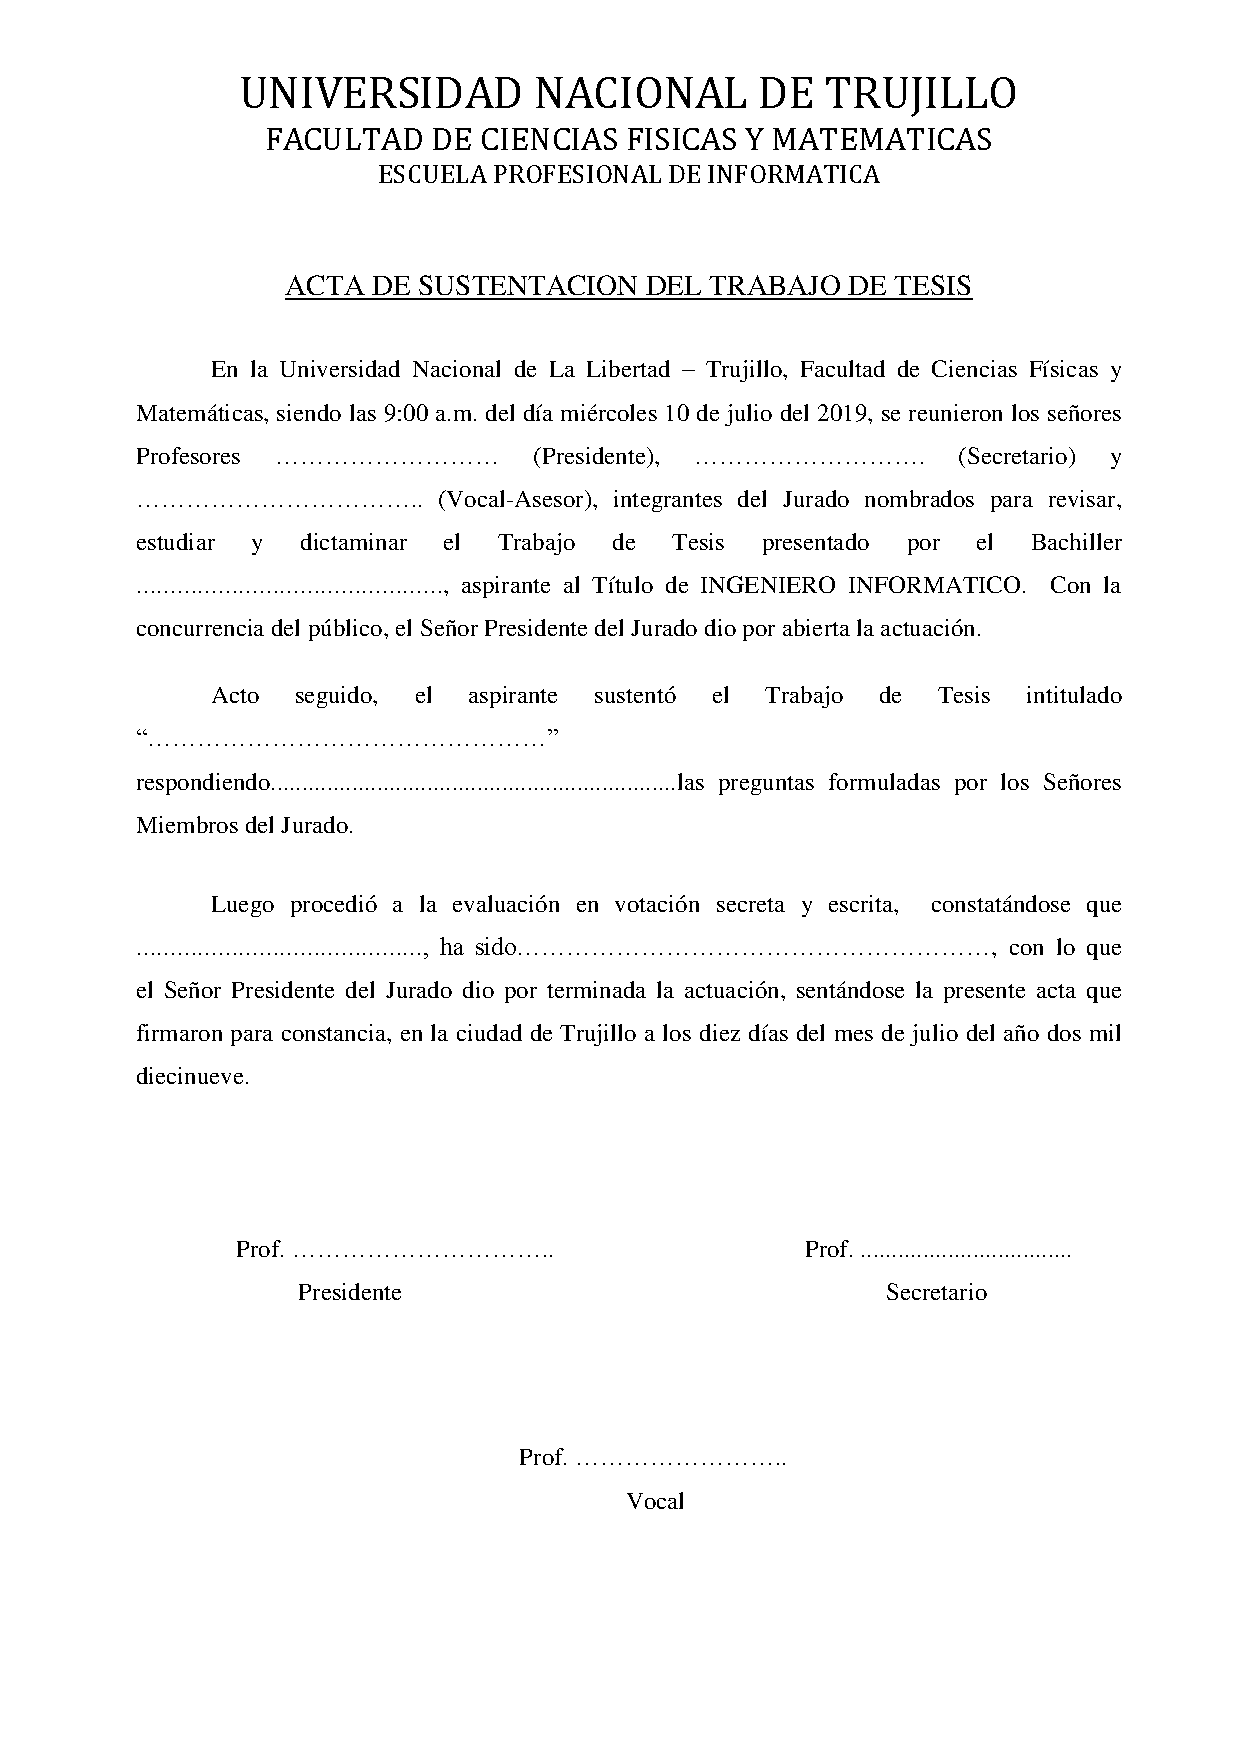
\includegraphics[scale=0.9]{Acta_Sustentacion.pdf}
\end{figure}
\includepdf[pagecommand={},width=\textwidth {Acta_Sustentacion.pdf}


%%%%%%%%%%%%%%%%%%%%%%%%%%%%%%%%%%%%%%%%%%%%%%%%%%%%%%%%%%%%%%%%%%%

%%%%%%%%%%%%%%%%%%%%%%%%%%%% RESUMEN%%%%%%%%%%%%%%%%%%%%%%
\newpage
\begin{center}
 \addcontentsline{toc}{chapter}{Resumen}
 {\bf\LARGE Resumen}
\end{center} 
\vskip 0.5cm
\begin{quotation}
Actualmente ...
\vskip 0.3cm
\hspace*{-0.6cm}{\bf Palabras claves:} redes neuronales, pronostico, sistemas basado en conocimiento.
\end{quotation}
%%%%%%%%%%%%%%%%%%%%%%%%%%%%%%%%%%%%%%%%%%%%%%%%%%%%%%%%%%%%%%%%%%%%%%%%%%%%%%%%%%%%


%%%%%%%%%%%%%%%%%%%%%%%%%%%%ABSTRACT%%%%%%%%%%%%%%%%%%%%%%
\newpage
\begin{center}
 \addcontentsline{toc}{chapter}{Abstract}
 {\bf\LARGE Abstract}\vskip 1.5cm
\end{center} 
\begin{quotation}
Currently ...
\vskip 0.3cm
\hspace*{-0.6cm}{\bf Keywords:} neural networks, , intelligent systems.
\end{quotation}
%%%%%%%%%%%%%%%%%%%%%%%%%%%%%%%%%%%%%%%%%%%%%%%%%%%%%%%%%%%%%%%%%%%%%%%%%%%%%%


%%%%%%%%%%%%%%%%%%%%%%%%%%%% LISTA DE SIMBOLOS %%%%%%%%%%%%%%%%%%%%%%
\newpage
\addcontentsline{toc}{chapter}{Lista de símbolos}
 {\bf\LARGE Lista de símbolos}
 \vskip 1.5cm
Constantes: 
\begin{enumerate}
\item[(1)]$r,\overline{r} $ \hspace*{0.8cm} Indice que denota regiones.
\item[(2)] $n $ \hspace*{1.1cm} Indice de bienes finales deseados por los consumidores.
\item[(3)] ...
\vskip 3cm
\end{enumerate} 
\vskip 0.3cm
Variables:
\begin{enumerate}
\item[(5)] $ x^{r} $ \hspace*{1cm} Vector columna que denota la actividad de producción.
\item[(6)] $ u^{r} $ \hspace*{1.2cm} . . .
\end{enumerate}

              % Datos de la tesis
\listoffigures               % indice de figuras
\addcontentsline{toc}{chapter}{Índice de Figuras}
\listoftables                % indice de tablas
\addcontentsline{toc}{chapter}{Índice de Tablas}
\tableofcontents             % indice de materias
\include{Caps}                % Capitulos de la tesis


\appendix
\chapter{Dataset de entrenamiento}
\begin{longtable} {|c|c|c|c|}
\hline
Año                      & Mes                                                                                                                                                                                                   & Día                                                 &
 \begin{tabular}[c]{@{}c@{}}Ventas\\ Observadas\end{tabular} \\     \hline
2018         & 1            & 10           & 1                         \\ 
\hline
2018         & 1            & 11           & 0                         \\ 
\hline
2018         & 1            & 12           & 0                         \\ 
\hline
2018         & 1            & 13           & 0                         \\ 
\hline
2018         & 1            & 14           & 0                         \\ 
\hline
2018         & 1            & 15           & 0                         \\ 
\hline
2018         & 1            & 16           & 0                         \\ 
\hline
2018         & 1            & 17           & 0                         \\ 
\hline
2018         & 1            & 18           & 0                         \\ 
\hline
2018         & 1            & 19           & 0                         \\ 
\hline
2018         & 1            & 20           & 0                         \\ 
\hline
2018         & 1            & 21           & 0                         \\ 
\hline
2018         & 1            & 22           & 0                         \\ 
\hline
2018         & 1            & 23           & 0                         \\ 
\hline
2018         & 1            & 24           & 0                         \\ 
\hline
2018         & 1            & 25           & 0                         \\ 
\hline
2018         & 1            & 26           & 0                         \\ 
\hline
2018         & 1            & 27           & 0                         \\ 
\hline
2018         & 1            & 28           & 0                         \\ 
\hline
2018         & 1            & 29           & 0                         \\ 
\hline
2018         & 1            & 30           & 0                         \\ 
\hline
2018         & 1            & 31           & 0                         \\ 
\hline
2018         & 2            & 1            & 1                         \\ 
\hline
2018         & 2            & 2            & 0                         \\ 
\hline
2018         & 2            & 3            & 0                         \\ 
\hline
2018         & 2            & 4            & 0                         \\ 
\hline
2018         & 2            & 5            & 0                         \\ 
\hline
2018         & 2            & 6            & 0                         \\ 
\hline
2018         & 2            & 7            & 0                         \\ 
\hline
2018         & 2            & 8            & 0                         \\ 
\hline
2018         & 2            & 9            & 0                         \\ 
\hline
2018         & 2            & 10           & 0                         \\ 
\hline
2018         & 2            & 11           & 0                         \\ 
\hline
2018         & 2            & 12           & 0                         \\ 
\hline
2018         & 2            & 13           & 0                         \\ 
\hline
2018         & 2            & 14           & 0                         \\ 
\hline
2018         & 2            & 15           & 0                         \\ 
\hline
2018         & 2            & 16           & 0                         \\ 
\hline
2018         & 2            & 17           & 0                         \\ 
\hline
2018         & 2            & 18           & 0                         \\ 
\hline
2018         & 2            & 19           & 0                         \\ 
\hline
2018         & 2            & 20           & 0                         \\ 
\hline
2018         & 2            & 21           & 0                         \\ 
\hline
2018         & 2            & 22           & 0                         \\ 
\hline
2018         & 2            & 23           & 0                         \\ 
\hline
2018         & 2            & 24           & 0                         \\ 
\hline
2018         & 2            & 25           & 0                         \\ 
\hline
2018         & 2            & 26           & 0                         \\ 
\hline
2018         & 2            & 27           & 0                         \\ 
\hline
2018         & 2            & 28           & 0                         \\ 
\hline
2018         & 3            & 1            & 0                         \\ 
\hline
2018         & 3            & 2            & 0                         \\ 
\hline
2018         & 3            & 3            & 0                         \\ 
\hline
2018         & 3            & 4            & 0                         \\ 
\hline
2018         & 3            & 5            & 0                         \\ 
\hline
2018         & 3            & 6            & 0                         \\ 
\hline
2018         & 3            & 7            & 0                         \\ 
\hline
2018         & 3            & 8            & 0                         \\ 
\hline
2018         & 3            & 9            & 0                         \\ 
\hline
2018         & 3            & 10           & 0                         \\ 
\hline
2018         & 3            & 11           & 0                         \\ 
\hline
2018         & 3            & 12           & 0                         \\ 
\hline
2018         & 3            & 13           & 0                         \\ 
\hline
2018         & 3            & 14           & 0                         \\ 
\hline
2018         & 3            & 15           & 0                         \\ 
\hline
2018         & 3            & 16           & 0                         \\ 
\hline
2018         & 3            & 17           & 0                         \\ 
\hline
2018         & 3            & 18           & 0                         \\ 
\hline
2018         & 3            & 19           & 0                         \\ 
\hline
2018         & 3            & 20           & 0                         \\ 
\hline
2018         & 3            & 21           & 0                         \\ 
\hline
2018         & 3            & 22           & 0                         \\ 
\hline
2018         & 3            & 23           & 0                         \\ 
\hline
2018         & 3            & 24           & 0                         \\ 
\hline
2018         & 3            & 25           & 0                         \\ 
\hline
2018         & 3            & 26           & 0                         \\ 
\hline
2018         & 3            & 27           & 0                         \\ 
\hline
2018         & 3            & 28           & 0                         \\ 
\hline
2018         & 3            & 29           & 0                         \\ 
\hline
2018         & 3            & 30           & 0                         \\ 
\hline
2018         & 3            & 31           & 0                         \\ 
\hline
2018         & 4            & 1            & 0                         \\ 
\hline
2018         & 4            & 2            & 0                         \\ 
\hline
2018         & 4            & 3            & 9                         \\ 
\hline
2018         & 4            & 4            & 26                        \\ 
\hline
2018         & 4            & 5            & 18                        \\ 
\hline
2018         & 4            & 6            & 9                         \\ 
\hline
2018         & 4            & 7            & 20                        \\ 
\hline
2018         & 4            & 8            & 32                        \\ 
\hline
2018         & 4            & 9            & 23                        \\ 
\hline
2018         & 4            & 10           & 23                        \\ 
\hline
2018         & 4            & 11           & 22                        \\ 
\hline
2018         & 4            & 12           & 15                        \\ 
\hline
2018         & 4            & 13           & 43                        \\ 
\hline
2018         & 4            & 14           & 23                        \\ 
\hline
2018         & 4            & 15           & 26                        \\ 
\hline
2018         & 4            & 16           & 30                        \\ 
\hline
2018         & 4            & 17           & 18                        \\ 
\hline
2018         & 4            & 18           & 19                        \\ 
\hline
2018         & 4            & 19           & 24                        \\ 
\hline
2018         & 4            & 20           & 18                        \\ 
\hline
2018         & 4            & 21           & 17                        \\ 
\hline
2018         & 4            & 22           & 32                        \\ 
\hline
2018         & 4            & 23           & 24                        \\ 
\hline
2018         & 4            & 24           & 27                        \\ 
\hline
2018         & 4            & 25           & 22                        \\ 
\hline
2018         & 4            & 26           & 27                        \\ 
\hline
2018         & 4            & 27           & 16                        \\ 
\hline
2018         & 4            & 28           & 23                        \\ 
\hline
2018         & 4            & 29           & 32                        \\ 
\hline
2018         & 4            & 30           & 0                         \\ 
\hline
2018         & 5            & 1            & 20                        \\ 
\hline
2018         & 5            & 2            & 27                        \\ 
\hline
2018         & 5            & 3            & 20                        \\ 
\hline
2018         & 5            & 4            & 12                        \\ 
\hline
2018         & 5            & 5            & 13                        \\ 
\hline
2018         & 5            & 6            & 33                        \\ 
\hline
2018         & 5            & 7            & 0                         \\ 
\hline
2018         & 5            & 8            & 20                        \\ 
\hline
2018         & 5            & 9            & 30                        \\ 
\hline
2018         & 5            & 10           & 19                        \\ 
\hline
2018         & 5            & 11           & 17                        \\ 
\hline
2018         & 5            & 12           & 22                        \\ 
\hline
2018         & 5            & 13           & 21                        \\ 
\hline
2018         & 5            & 14           & 0                         \\ 
\hline
2018         & 5            & 15           & 14                        \\ 
\hline
2018         & 5            & 16           & 17                        \\ 
\hline
2018         & 5            & 17           & 20                        \\ 
\hline
2018         & 5            & 18           & 24                        \\ 
\hline
2018         & 5            & 19           & 11                        \\ 
\hline
2018         & 5            & 20           & 29                        \\ 
\hline
2018         & 5            & 21           & 0                         \\ 
\hline
2018         & 5            & 22           & 16                        \\ 
\hline
2018         & 5            & 23           & 23                        \\ 
\hline
2018         & 5            & 24           & 14                        \\ 
\hline
2018         & 5            & 25           & 10                        \\ 
\hline
2018         & 5            & 26           & 20                        \\ 
\hline
2018         & 5            & 27           & 20                        \\ 
\hline
2018         & 5            & 28           & 0                         \\ 
\hline
2018         & 5            & 29           & 23                        \\ 
\hline
2018         & 5            & 30           & 26                        \\ 
\hline
2018         & 5            & 31           & 39                        \\ 
\hline
2018         & 6            & 1            & 23                        \\ 
\hline
2018         & 6            & 2            & 29                        \\ 
\hline
2018         & 6            & 3            & 39                        \\ 
\hline
2018         & 6            & 4            & 10                        \\ 
\hline
2018         & 6            & 5            & 15                        \\ 
\hline
2018         & 6            & 6            & 35                        \\ 
\hline
2018         & 6            & 7            & 25                        \\ 
\hline
2018         & 6            & 8            & 36                        \\ 
\hline
2018         & 6            & 9            & 41                        \\ 
\hline
2018         & 6            & 10           & 16                        \\ 
\hline
2018         & 6            & 11           & 20                        \\ 
\hline
2018         & 6            & 12           & 11                        \\ 
\hline
2018         & 6            & 13           & 19                        \\ 
\hline
2018         & 6            & 14           & 18                        \\ 
\hline
2018         & 6            & 15           & 20                        \\ 
\hline
2018         & 6            & 16           & 30                        \\ 
\hline
2018         & 6            & 17           & 35                        \\ 
\hline
2018         & 6            & 18           & 42                        \\ 
\hline
2018         & 6            & 19           & 8                         \\ 
\hline
2018         & 6            & 20           & 15                        \\ 
\hline
2018         & 6            & 21           & 24                        \\ 
\hline
2018         & 6            & 22           & 17                        \\ 
\hline
2018         & 6            & 23           & 34                        \\ 
\hline
2018         & 6            & 24           & 31                        \\ 
\hline
2018         & 6            & 25           & 21                        \\ 
\hline
2018         & 6            & 26           & 9                         \\ 
\hline
2018         & 6            & 27           & 32                        \\ 
\hline
2018         & 6            & 28           & 30                        \\ 
\hline
2018         & 6            & 29           & 23                        \\ 
\hline
2018         & 6            & 30           & 35                        \\ 
\hline
2018         & 7            & 1            & 28                        \\ 
\hline
2018         & 7            & 2            & 15                        \\ 
\hline
2018         & 7            & 3            & 11                        \\ 
\hline
2018         & 7            & 4            & 26                        \\ 
\hline
2018         & 7            & 5            & 23                        \\ 
\hline
2018         & 7            & 6            & 24                        \\ 
\hline
2018         & 7            & 7            & 21                        \\ 
\hline
2018         & 7            & 8            & 31                        \\ 
\hline
2018         & 7            & 9            & 19                        \\ 
\hline
2018         & 7            & 10           & 11                        \\ 
\hline
2018         & 7            & 11           & 22                        \\ 
\hline
2018         & 7            & 12           & 22                        \\ 
\hline
2018         & 7            & 13           & 17                        \\ 
\hline
2018         & 7            & 14           & 20                        \\ 
\hline
2018         & 7            & 15           & 25                        \\ 
\hline
2018         & 7            & 16           & 13                        \\ 
\hline
2018         & 7            & 17           & 11                        \\ 
\hline
2018         & 7            & 18           & 21                        \\ 
\hline
2018         & 7            & 19           & 11                        \\ 
\hline
2018         & 7            & 20           & 25                        \\ 
\hline
2018         & 7            & 21           & 25                        \\ 
\hline
2018         & 7            & 22           & 30                        \\ 
\hline
2018         & 7            & 23           & 13                        \\ 
\hline
2018         & 7            & 24           & 14                        \\ 
\hline
2018         & 7            & 25           & 19                        \\ 
\hline
2018         & 7            & 26           & 17                        \\ 
\hline
2018         & 7            & 27           & 19                        \\ 
\hline
2018         & 7            & 28           & 28                        \\ 
\hline
2018         & 7            & 29           & 40                        \\ 
\hline
2018         & 7            & 30           & 20                        \\ 
\hline
2018         & 7            & 31           & 9                         \\ 
\hline
2018         & 8            & 1            & 16                        \\ 
\hline
2018         & 8            & 2            & 16                        \\ 
\hline
2018         & 8            & 3            & 15                        \\ 
\hline
2018         & 8            & 4            & 29                        \\ 
\hline
2018         & 8            & 5            & 24                        \\ 
\hline
2018         & 8            & 6            & 22                        \\ 
\hline
2018         & 8            & 7            & 9                         \\ 
\hline
2018         & 8            & 8            & 17                        \\ 
\hline
2018         & 8            & 9            & 9                         \\ 
\hline
2018         & 8            & 10           & 11                        \\ 
\hline
2018         & 8            & 11           & 21                        \\ 
\hline
2018         & 8            & 12           & 23                        \\ 
\hline
2018         & 8            & 13           & 21                        \\ 
\hline
2018         & 8            & 14           & 5                         \\ 
\hline
2018         & 8            & 15           & 25                        \\ 
\hline
2018         & 8            & 16           & 19                        \\ 
\hline
2018         & 8            & 17           & 20                        \\ 
\hline
2018         & 8            & 18           & 21                        \\ 
\hline
2018         & 8            & 19           & 29                        \\ 
\hline
2018         & 8            & 20           & 38                        \\ 
\hline
2018         & 8            & 21           & 6                         \\ 
\hline
2018         & 8            & 22           & 24                        \\ 
\hline
2018         & 8            & 23           & 20                        \\ 
\hline
2018         & 8            & 24           & 20                        \\ 
\hline
2018         & 8            & 25           & 20                        \\ 
\hline
2018         & 8            & 26           & 38                        \\ 
\hline
2018         & 8            & 27           & 32                        \\ 
\hline
2018         & 8            & 28           & 12                        \\ 
\hline
2018         & 8            & 29           & 13                        \\ 
\hline
2018         & 8            & 30           & 25                        \\ 
\hline
2018         & 8            & 31           & 28                        \\ 
\hline
2018         & 9            & 1            & 33                        \\ 
\hline
2018         & 9            & 2            & 33                        \\ 
\hline
2018         & 9            & 3            & 30                        \\ 
\hline
2018         & 9            & 4            & 10                        \\ 
\hline
2018         & 9            & 5            & 16                        \\ 
\hline
2018         & 9            & 6            & 20                        \\ 
\hline
2018         & 9            & 7            & 18                        \\ 
\hline
2018         & 9            & 8            & 28                        \\ 
\hline
2018         & 9            & 9            & 26                        \\ 
\hline
2018         & 9            & 10           & 19                        \\ 
\hline
2018         & 9            & 11           & 4                         \\ 
\hline
2018         & 9            & 12           & 20                        \\ 
\hline
2018         & 9            & 13           & 25                        \\ 
\hline
2018         & 9            & 14           & 20                        \\ 
\hline
2018         & 9            & 15           & 25                        \\ 
\hline
2018         & 9            & 16           & 23                        \\ 
\hline
2018         & 9            & 17           & 17                        \\ 
\hline
2018         & 9            & 18           & 8                         \\ 
\hline
2018         & 9            & 19           & 20                        \\ 
\hline
2018         & 9            & 20           & 19                        \\ 
\hline
2018         & 9            & 21           & 20                        \\ 
\hline
2018         & 9            & 22           & 21                        \\ 
\hline
2018         & 9            & 23           & 28                        \\ 
\hline
2018         & 9            & 24           & 22                        \\ 
\hline
2018         & 9            & 25           & 7                         \\ 
\hline
2018         & 9            & 26           & 20                        \\ 
\hline
2018         & 9            & 27           & 22                        \\ 
\hline
2018         & 9            & 28           & 29                        \\ 
\hline
2018         & 9            & 29           & 23                        \\ 
\hline
2018         & 9            & 30           & 36                        \\ 
\hline
2018         & 10           & 1            & 21                        \\ 
\hline
2018         & 10           & 2            & 9                         \\ 
\hline
2018         & 10           & 3            & 15                        \\ 
\hline
2018         & 10           & 4            & 17                        \\ 
\hline
2018         & 10           & 5            & 20                        \\ 
\hline
2018         & 10           & 6            & 19                        \\ 
\hline
2018         & 10           & 7            & 28                        \\ 
\hline
2018         & 10           & 8            & 24                        \\ 
\hline
2018         & 10           & 9            & 0                         \\ 
\hline
2018         & 10           & 10           & 21                        \\ 
\hline
2018         & 10           & 11           & 13                        \\ 
\hline
2018         & 10           & 12           & 20                        \\ 
\hline
2018         & 10           & 13           & 14                        \\ 
\hline
2018         & 10           & 14           & 34                        \\ 
\hline
2018         & 10           & 15           & 22                        \\ 
\hline
2018         & 10           & 16           & 5                         \\ 
\hline
2018         & 10           & 17           & 15                        \\ 
\hline
2018         & 10           & 18           & 16                        \\ 
\hline
2018         & 10           & 19           & 11                        \\ 
\hline
2018         & 10           & 20           & 13                        \\ 
\hline
2018         & 10           & 21           & 22                        \\ 
\hline
2018         & 10           & 22           & 0                         \\ 
\hline
2018         & 10           & 23           & 26                        \\ 
\hline
2018         & 10           & 24           & 15                        \\ 
\hline
2018         & 10           & 25           & 22                        \\ 
\hline
2018         & 10           & 26           & 15                        \\ 
\hline
2018         & 10           & 27           & 16                        \\ 
\hline
2018         & 10           & 28           & 13                        \\ 
\hline
2018         & 10           & 29           & 0                         \\ 
\hline
2018         & 10           & 30           & 28                        \\ 
\hline
2018         & 10           & 31           & 12                        \\ 
\hline
2018         & 11           & 1            & 19                        \\ 
\hline
2018         & 11           & 2            & 26                        \\ 
\hline
2018         & 11           & 3            & 21                        \\ 
\hline
2018         & 11           & 4            & 22                        \\ 
\hline
2018         & 11           & 5            & 0                         \\ 
\hline
2018         & 11           & 6            & 22                        \\ 
\hline
2018         & 11           & 7            & 15                        \\ 
\hline
2018         & 11           & 8            & 13                        \\ 
\hline
2018         & 11           & 9            & 17                        \\ 
\hline
2018         & 11           & 10           & 24                        \\ 
\hline
2018         & 11           & 11           & 18                        \\ 
\hline
2018         & 11           & 12           & 0                         \\ 
\hline
2018         & 11           & 13           & 23                        \\ 
\hline
2018         & 11           & 14           & 14                        \\ 
\hline
2018         & 11           & 15           & 19                        \\ 
\hline
2018         & 11           & 16           & 20                        \\ 
\hline
2018         & 11           & 17           & 19                        \\ 
\hline
2018         & 11           & 18           & 24                        \\ 
\hline
2018         & 11           & 19           & 0                         \\ 
\hline
2018         & 11           & 20           & 27                        \\ 
\hline
2018         & 11           & 21           & 18                        \\ 
\hline
2018         & 11           & 22           & 19                        \\ 
\hline
2018         & 11           & 23           & 26                        \\ 
\hline
2018         & 11           & 24           & 17                        \\ 
\hline
2018         & 11           & 25           & 16                        \\ 
\hline
2018         & 11           & 26           & 0                         \\ 
\hline
2018         & 11           & 27           & 27                        \\ 
\hline
2018         & 11           & 28           & 14                        \\ 
\hline
2018         & 11           & 29           & 11                        \\ 
\hline
2018         & 11           & 30           & 19                        \\ 
\hline
2018         & 12           & 1            & 13                        \\ 
\hline
2018         & 12           & 2            & 24                        \\ 
\hline
2018         & 12           & 3            & 0                         \\ 
\hline
2018         & 12           & 4            & 20                        \\ 
\hline
2018         & 12           & 5            & 21                        \\ 
\hline
2018         & 12           & 6            & 16                        \\ 
\hline
2018         & 12           & 7            & 16                        \\ 
\hline
2018         & 12           & 8            & 26                        \\ 
\hline
2018         & 12           & 9            & 23                        \\ 
\hline
2018         & 12           & 10           & 0                         \\ 
\hline
2018         & 12           & 11           & 35                        \\ 
\hline
2018         & 12           & 12           & 25                        \\ 
\hline
2018         & 12           & 13           & 14                        \\ 
\hline
2018         & 12           & 14           & 18                        \\ 
\hline
2018         & 12           & 15           & 28                        \\ 
\hline
2018         & 12           & 16           & 32                        \\ 
\hline
2018         & 12           & 17           & 0                         \\ 
\hline
2018         & 12           & 18           & 29                        \\ 
\hline
2018         & 12           & 19           & 13                        \\ 
\hline
2018         & 12           & 20           & 17                        \\ 
\hline
2018         & 12           & 21           & 17                        \\ 
\hline
2018         & 12           & 22           & 20                        \\ 
\hline
2018         & 12           & 23           & 26                        \\ 
\hline
2018         & 12           & 24           & 0                         \\ 
\hline
2018         & 12           & 25           & 28                        \\ 
\hline
2018         & 12           & 26           & 36                        \\ 
\hline
2018         & 12           & 27           & 16                        \\ 
\hline
2018         & 12           & 28           & 20                        \\ 
\hline
2018         & 12           & 29           & 18                        \\ 
\hline
2018         & 12           & 30           & 28                        \\ 
\hline
2018         & 12           & 31           & 37                        \\ 
\hline
2019         & 1            & 1            & 21                        \\ 
\hline
2019         & 1            & 2            & 0                         \\ 
\hline
2019         & 1            & 3            & 38                        \\ 
\hline
2019         & 1            & 4            & 21                        \\ 
\hline
2019         & 1            & 5            & 21                        \\ 
\hline
2019         & 1            & 6            & 20                        \\ 
\hline
2019         & 1            & 7            & 0                         \\ 
\hline
2019         & 1            & 8            & 16                        \\ 
\hline
2019         & 1            & 9            & 16                        \\ 
\hline
2019         & 1            & 10           & 19                        \\ 
\hline
2019         & 1            & 11           & 21                        \\ 
\hline
2019         & 1            & 12           & 18                        \\ 
\hline
2019         & 1            & 13           & 19                        \\ 
\hline
2019         & 1            & 14           & 25                        \\ 
\hline
2019         & 1            & 15           & 15                        \\ 
\hline
2019         & 1            & 16           & 12                        \\ 
\hline
2019         & 1            & 17           & 6                         \\ 
\hline
2019         & 1            & 18           & 13                        \\ 
\hline
2019         & 1            & 19           & 16                        \\ 
\hline
2019         & 1            & 20           & 27                        \\ 
\hline
2019         & 1            & 21           & 27                        \\ 
\hline
2019         & 1            & 22           & 17                        \\ 
\hline
2019         & 1            & 23           & 13                        \\ 
\hline
2019         & 1            & 24           & 14                        \\ 
\hline
2019         & 1            & 25           & 14                        \\ 
\hline
2019         & 1            & 26           & 13                        \\ 
\hline
2019         & 1            & 27           & 22                        \\ 
\hline
2019         & 1            & 28           & 27                        \\ 
\hline
2019         & 1            & 29           & 9                         \\ 
\hline
2019         & 1            & 30           & 12                        \\ 
\hline
2019         & 1            & 31           & 18                        \\ 
\hline
2019         & 2            & 1            & 10                        \\ 
\hline
2019         & 2            & 2            & 15                        \\ 
\hline
2019         & 2            & 3            & 20                        \\ 
\hline
2019         & 2            & 4            & 25                        \\ 
\hline
2019         & 2            & 5            & 17                        \\ 
\hline
2019         & 2            & 6            & 12                        \\ 
\hline
2019         & 2            & 7            & 21                        \\ 
\hline
2019         & 2            & 8            & 14                        \\ 
\hline
2019         & 2            & 9            & 6                         \\ 
\hline
2019         & 2            & 10           & 15                        \\ 
\hline
2019         & 2            & 11           & 25                        \\ 
\hline
2019         & 2            & 12           & 9                         \\ 
\hline
2019         & 2            & 13           & 13                        \\ 
\hline
2019         & 2            & 14           & 20                        \\ 
\hline
2019         & 2            & 15           & 17                        \\ 
\hline
2019         & 2            & 16           & 10                        \\ 
\hline
2019         & 2            & 17           & 20                        \\ 
\hline
2019         & 2            & 18           & 25                        \\ 
\hline
2019         & 2            & 19           & 9                         \\ 
\hline
2019         & 2            & 20           & 5                         \\ 
\hline
2019         & 2            & 21           & 20                        \\ 
\hline
2019         & 2            & 22           & 8                         \\ 
\hline
2019         & 2            & 23           & 13                        \\ 
\hline
2019         & 2            & 24           & 16                        \\ 
\hline
2019         & 2            & 25           & 21                        \\ 
\hline
2019         & 2            & 26           & 13                        \\ 
\hline
2019         & 2            & 27           & 11                        \\ 
\hline
2019         & 2            & 28           & 14                        \\ 
\hline
2019         & 3            & 1            & 11                        \\ 
\hline
2019         & 3            & 2            & 11                        \\ 
\hline
2019         & 3            & 3            & 10                        \\ 
\hline
2019         & 3            & 4            & 25                        \\ 
\hline
2019         & 3            & 5            & 21                        \\ 
\hline
2019         & 3            & 6            & 11                        \\ 
\hline
2019         & 3            & 7            & 12                        \\ 
\hline
2019         & 3            & 8            & 9                         \\ 
\hline
2019         & 3            & 9            & 10                        \\ 
\hline
2019         & 3            & 10           & 21                        \\ 
\hline
2019         & 3            & 11           & 15                        \\ 
\hline
2019         & 3            & 12           & 11                        \\ 
\hline
2019         & 3            & 13           & 9                         \\ 
\hline
2019         & 3            & 14           & 13                        \\ 
\hline
2019         & 3            & 15           & 11                        \\ 
\hline
2019         & 3            & 16           & 18                        \\ 
\hline
2019         & 3            & 17           & 23                        \\ 
\hline
2019         & 3            & 18           & 19                        \\ 
\hline
2019         & 3            & 19           & 3                         \\ 
\hline
2019         & 3            & 20           & 5                         \\ 
\hline
2019         & 3            & 21           & 12                        \\ 
\hline
2019         & 3            & 22           & 9                         \\ 
\hline
2019         & 3            & 23           & 10                        \\ 
\hline
2019         & 3            & 24           & 21                        \\ 
\hline
2019         & 3            & 25           & 16                        \\ 
\hline
2019         & 3            & 26           & 15                        \\ 
\hline
2019         & 3            & 27           & 7                         \\ 
\hline
2019         & 3            & 28           & 9                         \\ 
\hline
2019         & 3            & 29           & 7                         \\ 
\hline
2019         & 3            & 30           & 16                        \\ 
\hline
2019         & 3            & 31           & 20                        \\ 
\hline
2019         & 4            & 1            & 17                        \\ 
\hline
2019         & 4            & 2            & 0                         \\ 
\hline
2019         & 4            & 3            & 8                         \\ 
\hline
2019         & 4            & 4            & 9                         \\ 
\hline
2019         & 4            & 5            & 13                        \\ 
\hline
2019         & 4            & 6            & 5                         \\ 
\hline
2019         & 4            & 7            & 25                        \\ 
\hline
2019         & 4            & 8            & 23                        \\ 
\hline
2019         & 4            & 9            & 0                         \\ 
\hline
2019         & 4            & 10           & 0                         \\ 
\hline
2019         & 4            & 11           & 11                        \\ 
\hline
2019         & 4            & 12           & 8                         \\ 
\hline
2019         & 4            & 13           & 14                        \\ 
\hline
2019         & 4            & 14           & 12                        \\ 
\hline
2019         & 4            & 15           & 18                        \\ 
\hline
2019         & 4            & 16           & 7                         \\ 
\hline
2019         & 4            & 17           & 4                         \\ 
\hline
2019         & 4            & 18           & 18                        \\ 
\hline
2019         & 4            & 19           & 16                        \\ 
\hline
2019         & 4            & 20           & 19                        \\ 
\hline
2019         & 4            & 21           & 8                         \\ 
\hline
2019         & 4            & 22           & 19                        \\ 
\hline
2019         & 4            & 23           & 6                         \\ 
\hline
2019         & 4            & 24           & 9                         \\ 
\hline
2019         & 4            & 25           & 14                        \\ 
\hline
2019         & 4            & 26           & 7                         \\ 
\hline
2019         & 4            & 27           & 8                         \\ 
\hline
2019         & 4            & 28           & 19                        \\ 
\hline
2019         & 4            & 29           & 19                        \\ 
\hline
2019         & 4            & 30           & 7                         \\ 
\hline
2019         & 5            & 1            & 11                        \\ 
\hline
2019         & 5            & 2            & 17                        \\ 
\hline
2019         & 5            & 3            & 6                         \\ 
\hline
2019         & 5            & 4            & 7                         \\ 
\hline
2019         & 5            & 5            & 7                         \\ 
\hline
2019         & 5            & 6            & 21                        \\ 
\hline
2019         & 5            & 7            & 11                        \\ 
\hline
2019         & 5            & 8            & 10                        \\ 
\hline
2019         & 5            & 9            & 7                         \\ 
\hline
2019         & 5            & 10           & 9                         \\ 
\hline
2019         & 5            & 11           & 8                         \\ 
\hline
2019         & 5            & 12           & 14                        \\ 
\hline
2019         & 5            & 13           & 19                        \\ 
\hline
2019         & 5            & 14           & 10                        \\ 
\hline
2019         & 5            & 15           & 12                        \\ 
\hline
2019         & 5            & 16           & 7                         \\ 
\hline
2019         & 5            & 17           & 0                         \\ 
\hline
2019         & 5            & 18           & 3                         \\ 
\hline
2019         & 5            & 19           & 15                        \\ 
\hline
2019         & 5            & 20           & 19                        \\ 
\hline
2019         & 5            & 21           & 14                        \\ 
\hline
2019         & 5            & 22           & 8                         \\ 
\hline
2019         & 5            & 23           & 15                        \\ 
\hline
2019         & 5            & 24           & 6                         \\ 
\hline
2019         & 5            & 25           & 5                         \\ 
\hline
2019         & 5            & 26           & 11                        \\ 
\hline
2019         & 5            & 27           & 20                        \\ 
\hline
2019         & 5            & 28           & 10                        \\ 
\hline
2019         & 5            & 29           & 8                         \\ 
\hline
2019         & 5            & 30           & 19                        \\ 
\hline
2019         & 5            & 31           & 17                        \\ 
\hline
2019         & 6            & 1            & 11                        \\ 
\hline
2019         & 6            & 2            & 18                        \\ 
\hline
2019         & 6            & 3            & 14                        \\ 
\hline
2019         & 6            & 4            & 12                        \\ 
\hline
2019         & 6            & 5            & 8                         \\ 
\hline
2019         & 6            & 6            & 7                         \\ 
\hline
2019         & 6            & 7            & 7                         \\ 
\hline
2019         & 6            & 8            & 8                         \\ 
\hline
2019         & 6            & 9            & 16                        \\ 
\hline
2019         & 6            & 10           & 21                        \\ 
\hline
2019         & 6            & 11           & 0                         \\ 
\hline
2019         & 6            & 12           & 5                         \\ 
\hline
2019         & 6            & 13           & 18                        \\ 
\hline
2019         & 6            & 14           & 15                        \\ 
\hline
2019         & 6            & 15           & 15                        \\ 
\hline
2019         & 6            & 16           & 15                        \\ 
\hline
2019         & 6            & 17           & 11                        \\ 
\hline
2019         & 6            & 18           & 0                         \\ 
\hline
2019         & 6            & 19           & 7                         \\ 
\hline
2019         & 6            & 20           & 9                         \\ 
\hline
2019         & 6            & 21           & 4                         \\ 
\hline
2019         & 6            & 22           & 12                        \\ 
\hline
2019         & 6            & 23           & 16                        \\ 
\hline
2019         & 6            & 24           & 25                        \\ 
\hline
2019         & 6            & 25           & 9                         \\ 
\hline
2019         & 6            & 26           & 10                        \\ 
\hline
2019         & 6            & 27           & 9                         \\ 
\hline
2019         & 6            & 28           & 6                         \\ 
\hline
2019         & 6            & 29           & 6                         \\ 
\hline
2019         & 6            & 30           & 23                        \\ 
\hline
2019         & 7            & 1            & 12                        \\ 
\hline
2019         & 7            & 2            & 10                        \\ 
\hline
2019         & 7            & 3            & 5                         \\ 
\hline
2019         & 7            & 4            & 8                         \\ 
\hline
2019         & 7            & 5            & 9                         \\ 
\hline
2019         & 7            & 6            & 15                        \\ 
\hline
2019         & 7            & 7            & 15                        \\ 
\hline
2019         & 7            & 8            & 22                        \\ 
\hline
2019         & 7            & 9            & 5                         \\ 
\hline
2019         & 7            & 10           & 10                        \\ 
\hline
2019         & 7            & 11           & 7                         \\ 
\hline
2019         & 7            & 12           & 7                         \\ 
\hline
2019         & 7            & 13           & 8                         \\ 
\hline
2019         & 7            & 14           & 16                        \\ 
\hline
2019         & 7            & 15           & 24                        \\ 
\hline
2019         & 7            & 16           & 8                         \\ 
\hline
2019         & 7            & 17           & 10                        \\ 
\hline
2019         & 7            & 18           & 17                        \\ 
\hline
2019         & 7            & 19           & 12                        \\ 
\hline
2019         & 7            & 20           & 8                         \\ 
\hline
2019         & 7            & 21           & 20                        \\ 
\hline
2019         & 7            & 22           & 18                        \\ 
\hline
2019         & 7            & 23           & 7                         \\ 
\hline
2019         & 7            & 24           & 7                         \\ 
\hline
2019         & 7            & 25           & 7                         \\ 
\hline
2019         & 7            & 26           & 6                         \\ 
\hline
2019         & 7            & 27           & 7                         \\ 
\hline
2019         & 7            & 28           & 10                        \\ 
\hline
2019         & 7            & 29           & 12                        \\ 
\hline
2019         & 7            & 30           & 7                         \\ 
\hline
2019         & 7            & 31           & 3                         \\ 
\hline
2019         & 8            & 1            & 8                         \\ 
\hline
2019         & 8            & 2            & 6                         \\ 
\hline
2019         & 8            & 3            & 8                         \\ 
\hline
2019         & 8            & 4            & 18                        \\ 
\hline
2019         & 8            & 5            & 13                        \\ 
\hline
2019         & 8            & 6            & 6                         \\ 
\hline
2019         & 8            & 7            & 8                         \\ 
\hline
2019         & 8            & 8            & 7                         \\ 
\hline
2019         & 8            & 9            & 2                         \\ 
\hline
2019         & 8            & 10           & 5                         \\ 
\hline
2019         & 8            & 11           & 12                        \\ 
\hline
2019         & 8            & 12           & 12                        \\ 
\hline
2019         & 8            & 13           & 6                         \\ 
\hline
2019         & 8            & 14           & 9                         \\ 
\hline
2019         & 8            & 15           & 5                         \\ 
\hline
2019         & 8            & 16           & 3                         \\ 
\hline
2019         & 8            & 17           & 4                         \\ 
\hline
2019         & 8            & 18           & 14                        \\ 
\hline
2019         & 8            & 19           & 22                        \\ 
\hline
2019         & 8            & 20           & 4                         \\ 
\hline
2019         & 8            & 21           & 4                         \\ 
\hline
2019         & 8            & 22           & 7                         \\ 
\hline
2019         & 8            & 23           & 6                         \\ 
\hline
2019         & 8            & 24           & 4                         \\ 
\hline
2019         & 8            & 25           & 15                        \\ 
\hline
2019         & 8            & 26           & 20                        \\ 
\hline
2019         & 8            & 27           & 6                         \\ 
\hline
2019         & 8            & 28           & 13                        \\ 
\hline
2019         & 8            & 29           & 4                         \\ 
\hline
2019         & 8            & 30           & 7                         \\ 
\hline
2019         & 8            & 31           & 5                         \\ 
\hline
2019         & 9            & 1            & 15                        \\ 
\hline
2019         & 9            & 2            & 16                        \\ 
\hline
2019         & 9            & 3            & 4                         \\ 
\hline
2019         & 9            & 4            & 4                         \\ 
\hline
2019         & 9            & 5            & 7                         \\ 
\hline
2019         & 9            & 6            & 1                         \\ 
\hline
2019         & 9            & 7            & 16                        \\ 
\hline
2019         & 9            & 8            & 13                        \\ 
\hline
2019         & 9            & 9            & 19                        \\ 
\hline
2019         & 9            & 10           & 3                         \\ 
\hline
2019         & 9            & 11           & 1                         \\ 
\hline
2019         & 9            & 12           & 11                        \\ 
\hline
2019         & 9            & 13           & 3                         \\ 
\hline
2019         & 9            & 14           & 3                         \\ 
\hline
2019         & 9            & 15           & 18                        \\ 
\hline
2019         & 9            & 16           & 13                        \\ 
\hline
2019         & 9            & 17           & 5                         \\ 
\hline
2019         & 9            & 18           & 5                         \\ 
\hline
2019         & 9            & 19           & 3                         \\ 
\hline
2019         & 9            & 20           & 6                         \\ 
\hline
2019         & 9            & 21           & 7                         \\ 
\hline
2019         & 9            & 22           & 12                        \\ 
\hline
2019         & 9            & 23           & 16                        \\ 
\hline
2019         & 9            & 24           & 5                         \\ 
\hline
2019         & 9            & 25           & 5                         \\ 
\hline
2019         & 9            & 26           & 8                         \\ 
\hline
2019         & 9            & 27           & 10                        \\ 
\hline
2019         & 9            & 28           & 5                         \\ 
\hline
2019         & 9            & 29           & 11                        \\ 
\hline
2019         & 9            & 30           & 0                         \\ 
\hline
2019         & 10           & 1            & 21                        \\ 
\hline
2019         & 10           & 2            & 7                         \\ 
\hline
2019         & 10           & 3            & 6                         \\ 
\hline
2019         & 10           & 4            & 10                        \\ 
\hline
2019         & 10           & 5            & 5                         \\ 
\hline
2019         & 10           & 6            & 7                         \\ 
\hline
2019         & 10           & 7            & 13                        \\ 
\hline
2019         & 10           & 8            & 3                         \\ 
\hline
2019         & 10           & 9            & 5                         \\ 
\hline
2019         & 10           & 10           & 5                         \\ 
\hline
2019         & 10           & 11           & 10                        \\ 
\hline
2019         & 10           & 12           & 11                        \\ 
\hline
2019         & 10           & 13           & 10                        \\ 
\hline
2019         & 10           & 14           & 12                        \\ 
\hline
2019         & 10           & 15           & 6                         \\ 
\hline
2019         & 10           & 16           & 3                         \\ 
\hline
2019         & 10           & 17           & 4                         \\ 
\hline
2019         & 10           & 18           & 6                         \\ 
\hline
2019         & 10           & 19           & 3                         \\ 
\hline
2019         & 10           & 20           & 7                         \\ 
\hline
2019         & 10           & 21           & 9                         \\ 
\hline
2019         & 10           & 22           & 2                         \\ 
\hline
2019         & 10           & 23           & 6                         \\ 
\hline
2019         & 10           & 24           & 17                        \\ 
\hline
2019         & 10           & 25           & 15                        \\ 
\hline
2019         & 10           & 26           & 13                        \\ 
\hline
2019         & 10           & 27           & 26                        \\ 
\hline
2019         & 10           & 28           & 13                        \\ 
\hline
2019         & 10           & 29           & 22                        \\ 
\hline
2019         & 10           & 30           & 17                        \\ 
\hline
2019         & 10           & 31           & 9                         \\ 
\hline
2019         & 11           & 1            & 13                        \\ 
\hline
2019         & 11           & 2            & 14                        \\ 
\hline
2019         & 11           & 3            & 17                        \\ 
\hline
2019         & 11           & 4            & 20                        \\ 
\hline
2019         & 11           & 5            & 13                        \\ 
\hline
2019         & 11           & 6            & 0                         \\ 
\hline
2019         & 11           & 7            & 17                        \\ 
\hline
2019         & 11           & 8            & 11                        \\ 
\hline
2019         & 11           & 9            & 15                        \\ 
\hline
2019         & 11           & 10           & 20                        \\ 
\hline
2019         & 11           & 11           & 9                         \\ 
\hline
2019         & 11           & 12           & 14                        \\ 
\hline
2019         & 11           & 13           & 7                         \\ 
\hline
2019         & 11           & 14           & 8                         \\ 
\hline
2019         & 11           & 15           & 11                        \\ 
\hline
2019         & 11           & 16           & 15                        \\ 
\hline
2019         & 11           & 17           & 25                        \\ 
\hline
2019         & 11           & 18           & 12                        \\ 
\hline
2019         & 11           & 19           & 16                        \\ 
\hline
2019         & 11           & 20           & 13                        \\ 
\hline
2019         & 11           & 21           & 15                        \\ 
\hline
2019         & 11           & 22           & 13                        \\ 
\hline
2019         & 11           & 23           & 10                        \\ 
\hline
2019         & 11           & 24           & 19                        \\ 
\hline
2019         & 11           & 25           & 10                        \\ 
\hline
2019         & 11           & 26           & 12                        \\ 
\hline
2019         & 11           & 27           & 5                         \\ 
\hline
2019         & 11           & 28           & 14                        \\ 
\hline
2019         & 11           & 29           & 9                         \\ 
\hline
2019         & 11           & 30           & 11                        \\ 
\hline
2019         & 12           & 1            & 13                        \\ 
\hline
2019         & 12           & 2            & 20                        \\ 
\hline
2019         & 12           & 3            & 10                        \\ 
\hline
2019         & 12           & 4            & 1                         \\ 
\hline
2019         & 12           & 5            & 12                        \\ 
\hline
2019         & 12           & 6            & 6                         \\ 
\hline
2019         & 12           & 7            & 15                        \\ 
\hline
2019         & 12           & 8            & 9                         \\ 
\hline
2019         & 12           & 9            & 15                        \\ 
\hline
2019         & 12           & 10           & 7                         \\ 
\hline
2019         & 12           & 11           & 8                         \\ 
\hline
2019         & 12           & 12           & 5                         \\ 
\hline
2019         & 12           & 13           & 7                         \\ 
\hline
2019         & 12           & 14           & 7                         \\ 
\hline
2019         & 12           & 15           & 8                         \\ 
\hline
2019         & 12           & 16           & 17                        \\ 
\hline
2019         & 12           & 17           & 5                         \\ 
\hline
2019         & 12           & 18           & 4                         \\ 
\hline
2019         & 12           & 19           & 14                        \\ 
\hline
2019         & 12           & 20           & 11                        \\ 
\hline
2019         & 12           & 21           & 11                        \\ 
\hline
2019         & 12           & 22           & 20                        \\ 
\hline
2019         & 12           & 23           & 11                        \\ 
\hline
2019         & 12           & 24           & 9                         \\ 
\hline
2019         & 12           & 25           & 10                        \\ 
\hline
2019         & 12           & 26           & 11                        \\ 
\hline
2019         & 12           & 27           & 7                         \\ 
\hline
2019         & 12           & 28           & 12                        \\ 
\hline
2019         & 12           & 29           & 8                         \\ 
\hline
2019         & 12           & 30           & 8                         \\ 
\hline
2019         & 12           & 31           & 5                         \\ 
\hline
2020         & 1            & 1            & 9                         \\ 
\hline
2020         & 1            & 2            & 17                        \\ 
\hline
2020         & 1            & 3            & 13                        \\ 
\hline
2020         & 1            & 4            & 0                         \\ 
\hline
2020         & 1            & 5            & 17                        \\ 
\hline
2020         & 1            & 6            & 11                        \\ 
\hline
2020         & 1            & 7            & 7                         \\ 
\hline
2020         & 1            & 8            & 11                        \\ 
\hline
2020         & 1            & 9            & 12                        \\ 
\hline
2020         & 1            & 10           & 10                        \\ 
\hline
2020         & 1            & 11           & 8                         \\ 
\hline
2020         & 1            & 12           & 9                         \\ 
\hline
2020         & 1            & 13           & 0                         \\ 
\hline
2020         & 1            & 14           & 6                         \\ 
\hline
2020         & 1            & 15           & 6                         \\ 
\hline
2020         & 1            & 16           & 11                        \\ 
\hline
2020         & 1            & 17           & 8                         \\ 
\hline
2020         & 1            & 18           & 11                        \\ 
\hline
2020         & 1            & 19           & 4                         \\ 
\hline
2020         & 1            & 20           & 8                         \\ 
\hline
2020         & 1            & 21           & 0                         \\ 
\hline
2020         & 1            & 22           & 10                        \\ 
\hline
2020         & 1            & 23           & 9                         \\ 
\hline
2020         & 1            & 24           & 8                         \\ 
\hline
2020         & 1            & 25           & 5                         \\ 
\hline
2020         & 1            & 26           & 4                         \\ 
\hline
2020         & 1            & 27           & 12                        \\ 
\hline
2020         & 1            & 28           & 0                         \\ 
\hline
2020         & 1            & 29           & 8                         \\ 
\hline
2020         & 1            & 30           & 10                        \\ 
\hline
2020         & 1            & 31           & 9                         \\ 
\hline
2020         & 2            & 1            & 2                         \\ 
\hline
2020         & 2            & 2            & 7                         \\ 
\hline
2020         & 2            & 3            & 12                        \\ 
\hline
2020         & 2            & 4            & 0                         \\ 
\hline
2020         & 2            & 5            & 4                         \\ 
\hline
2020         & 2            & 6            & 0                         \\ 
\hline
2020         & 2            & 7            & 6                         \\ 
\hline
2020         & 2            & 8            & 4                         \\ 
\hline
2020         & 2            & 9            & 10                        \\ 
\hline
2020         & 2            & 10           & 6                         \\ 
\hline
2020         & 2            & 11           & 0                         \\ 
\hline
2020         & 2            & 12           & 3                         \\ 
\hline
2020         & 2            & 13           & 6                         \\ 
\hline
2020         & 2            & 14           & 4                         \\ 
\hline
2020         & 2            & 15           & 10                        \\ 
\hline
2020         & 2            & 16           & 15                        \\ 
\hline
2020         & 2            & 17           & 6                         \\ 
\hline
2020         & 2            & 18           & 4                         \\ 
\hline
2020         & 2            & 19           & 0                         \\ 
\hline
2020         & 2            & 20           & 3                         \\ 
\hline
2020         & 2            & 21           & 3                         \\ 
\hline
2020         & 2            & 22           & 3                         \\ 
\hline
2020         & 2            & 23           & 5                         \\ 
\hline
2020         & 2            & 24           & 0                         \\ 
\hline
2020         & 2            & 25           & 16                        \\ 
\hline
2020         & 2            & 26           & 5                         \\ 
\hline
2020         & 2            & 27           & 3                         \\ 
\hline
2020         & 2            & 28           & 2                         \\ 
\hline
2020         & 2            & 29           & 5                         \\ 
\hline
2020         & 3            & 1            & 6                         \\ 
\hline
2020         & 3            & 2            & 7                         \\ 
\hline
2020         & 3            & 3            & 0                         \\ 
\hline
2020         & 3            & 4            & 4                         \\ 
\hline
2020         & 3            & 5            & 1                         \\ 
\hline
2020         & 3            & 6            & 3                         \\ 
\hline
2020         & 3            & 7            & 2                         \\ 
\hline
2020         & 3            & 8            & 6                         \\ 
\hline
2020         & 3            & 9            & 5                         \\ 
\hline
2020         & 3            & 10           & 3                         \\ 
\hline
2020         & 3            & 11           & 6                         \\ 
\hline
2020         & 3            & 12           & 0                         \\ 
\hline
2020         & 3            & 13           & 3                         \\ 
\hline
2020         & 3            & 14           & 6                         \\ 
\hline
2020         & 3            & 15           & 3                         \\ 
\hline
2020         & 3            & 16           & 0                         \\ 
\hline
2020         & 3            & 17           & 0                         \\ 
\hline
2020         & 3            & 18           & 0                         \\ 
\hline
2020         & 3            & 19           & 0                         \\ 
\hline
2020         & 3            & 20           & 0                         \\ 
\hline
2020         & 3            & 21           & 0                         \\ 
\hline
2020         & 3            & 22           & 0                         \\ 
\hline
2020         & 3            & 23           & 0                         \\ 
\hline
2020         & 3            & 24           & 0                         \\ 
\hline
2020         & 3            & 25           & 0                         \\ 
\hline
2020         & 3            & 26           & 0                         \\ 
\hline
2020         & 3            & 27           & 0                         \\ 
\hline
2020         & 3            & 28           & 0                         \\ 
\hline
2020         & 3            & 29           & 0                         \\ 
\hline
2020         & 3            & 30           & 0                         \\ 
\hline
2020         & 3            & 31           & 0                         \\ 
\hline
2020         & 4            & 1            & 0                         \\ 
\hline
2020         & 4            & 2            & 0                         \\ 
\hline
2020         & 4            & 3            & 0                         \\ 
\hline
2020         & 4            & 4            & 0                         \\ 
\hline
2020         & 4            & 5            & 0                         \\ 
\hline
2020         & 4            & 6            & 0                         \\ 
\hline
2020         & 4            & 7            & 0                         \\ 
\hline
2020         & 4            & 8            & 0                         \\ 
\hline
2020         & 4            & 9            & 0                         \\ 
\hline
2020         & 4            & 10           & 0                         \\ 
\hline
2020         & 4            & 11           & 0                         \\ 
\hline
2020         & 4            & 12           & 0                         \\ 
\hline
2020         & 4            & 13           & 0                         \\ 
\hline
2020         & 4            & 14           & 0                         \\ 
\hline
2020         & 4            & 15           & 0                         \\ 
\hline
2020         & 4            & 16           & 0                         \\ 
\hline
2020         & 4            & 17           & 0                         \\ 
\hline
2020         & 4            & 18           & 0                         \\ 
\hline
2020         & 4            & 19           & 0                         \\ 
\hline
2020         & 4            & 20           & 0                         \\ 
\hline
2020         & 4            & 21           & 0                         \\ 
\hline
2020         & 4            & 22           & 0                         \\ 
\hline
2020         & 4            & 23           & 0                         \\ 
\hline
2020         & 4            & 24           & 0                         \\ 
\hline
2020         & 4            & 25           & 0                         \\ 
\hline
2020         & 4            & 26           & 0                         \\ 
\hline
2020         & 4            & 27           & 0                         \\ 
\hline
2020         & 4            & 28           & 0                         \\ 
\hline
2020         & 4            & 29           & 0                         \\ 
\hline
2020         & 4            & 30           & 0                         \\ 
\hline
2020         & 5            & 1            & 0                         \\ 
\hline
2020         & 5            & 2            & 0                         \\ 
\hline
2020         & 5            & 3            & 0                         \\ 
\hline
2020         & 5            & 4            & 0                         \\ 
\hline
2020         & 5            & 5            & 0                         \\ 
\hline
2020         & 5            & 6            & 0                         \\ 
\hline
2020         & 5            & 7            & 0                         \\ 
\hline
2020         & 5            & 8            & 0                         \\ 
\hline
2020         & 5            & 9            & 0                         \\ 
\hline
2020         & 5            & 10           & 0                         \\ 
\hline
2020         & 5            & 11           & 0                         \\ 
\hline
2020         & 5            & 12           & 0                         \\ 
\hline
2020         & 5            & 13           & 0                         \\ 
\hline
2020         & 5            & 14           & 0                         \\ 
\hline
2020         & 5            & 15           & 7                         \\ 
\hline
2020         & 5            & 16           & 4                         \\ 
\hline
2020         & 5            & 17           & 0                         \\ 
\hline
2020         & 5            & 18           & 6                         \\ 
\hline
2020         & 5            & 19           & 4                         \\ 
\hline
2020         & 5            & 20           & 8                         \\ 
\hline
2020         & 5            & 21           & 8                         \\ 
\hline
2020         & 5            & 22           & 6                         \\ 
\hline
2020         & 5            & 23           & 7                         \\ 
\hline
2020         & 5            & 24           & 0                         \\ 
\hline
2020         & 5            & 25           & 4                         \\ 
\hline
2020         & 5            & 26           & 8                         \\ 
\hline
2020         & 5            & 27           & 3                         \\ 
\hline
2020         & 5            & 28           & 4                         \\ 
\hline
2020         & 5            & 29           & 8                         \\ 
\hline
2020         & 5            & 30           & 4                         \\ 
\hline
2020         & 5            & 31           & 0                         \\ 
\hline
2020         & 6            & 1            & 2                         \\ 
\hline
2020         & 6            & 2            & 3                         \\ 
\hline
2020         & 6            & 3            & 6                         \\ 
\hline
2020         & 6            & 4            & 6                         \\ 
\hline
2020         & 6            & 5            & 3                         \\ 
\hline
2020         & 6            & 6            & 3                         \\ 
\hline
2020         & 6            & 7            & 0                         \\ 
\hline
2020         & 6            & 8            & 6                         \\ 
\hline
2020         & 6            & 9            & 6                         \\ 
\hline
2020         & 6            & 10           & 5                         \\ 
\hline
2020         & 6            & 11           & 5                         \\ 
\hline
2020         & 6            & 12           & 5                         \\ 
\hline
2020         & 6            & 13           & 6                         \\ 
\hline
2020         & 6            & 14           & 0                         \\ 
\hline
2020         & 6            & 15           & 13                        \\ 
\hline
2020         & 6            & 16           & 4                         \\ 
\hline
2020         & 6            & 17           & 1                         \\ 
\hline
2020         & 6            & 18           & 7                         \\ 
\hline
2020         & 6            & 19           & 4                         \\ 
\hline
2020         & 6            & 20           & 5                         \\ 
\hline
2020         & 6            & 21           & 6                         \\ 
\hline
2020         & 6            & 22           & 6                         \\ 
\hline
2020         & 6            & 23           & 4                         \\ 
\hline
2020         & 6            & 24           & 3                         \\ 
\hline
2020         & 6            & 25           & 2                         \\ 
\hline
2020         & 6            & 26           & 6                         \\ 
\hline
2020         & 6            & 27           & 5                         \\ 
\hline
2020         & 6            & 28           & 0                         \\ 
\hline
2020         & 6            & 29           & 7                         \\ 
\hline
2020         & 6            & 30           & 4                         \\ 
\hline
2020         & 7            & 1            & 4                         \\ 
\hline
2020         & 7            & 2            & 7                         \\ 
\hline
2020         & 7            & 3            & 4                         \\ 
\hline
2020         & 7            & 4            & 6                         \\ 
\hline
2020         & 7            & 5            & 7                         \\ 
\hline
2020         & 7            & 6            & 9                         \\ 
\hline
2020         & 7            & 7            & 6                         \\ 
\hline
2020         & 7            & 8            & 3                         \\ 
\hline
2020         & 7            & 9            & 7                         \\ 
\hline
2020         & 7            & 10           & 3                         \\ 
\hline
2020         & 7            & 11           & 5                         \\ 
\hline
2020         & 7            & 12           & 6                         \\ 
\hline
2020         & 7            & 13           & 6                         \\ 
\hline
2020         & 7            & 14           & 0                         \\ 
\hline
2020         & 7            & 15           & 4                         \\ 
\hline
2020         & 7            & 16           & 7                         \\ 
\hline
2020         & 7            & 17           & 4                         \\ 
\hline
2020         & 7            & 18           & 5                         \\ 
\hline
2020         & 7            & 19           & 4                         \\ 
\hline
2020         & 7            & 20           & 9                         \\ 
\hline
2020         & 7            & 21           & 1                         \\ 
\hline
2020         & 7            & 22           & 0                         \\ 
\hline
2020         & 7            & 23           & 3                         \\ 
\hline
2020         & 7            & 24           & 4                         \\ 
\hline
2020         & 7            & 25           & 4                         \\ 
\hline
2020         & 7            & 26           & 7                         \\ 
\hline
2020         & 7            & 27           & 0                         \\ 
\hline
2020         & 7            & 28           & 12                        \\ 
\hline
2020         & 7            & 29           & 7                         \\ 
\hline
2020         & 7            & 30           & 0                         \\ 
\hline
2020         & 7            & 31           & 3                         \\ 
\hline
2020         & 8            & 1            & 6                         \\ 
\hline
2020         & 8            & 2            & 7                         \\ 
\hline
2020         & 8            & 3            & 8                         \\ 
\hline
2020         & 8            & 4            & 2                         \\ 
\hline
2020         & 8            & 5            & 1                         \\ 
\hline
2020         & 8            & 6            & 0                         \\ 
\hline
2020         & 8            & 7            & 2                         \\ 
\hline
2020         & 8            & 8            & 2                         \\ 
\hline
2020         & 8            & 9            & 6                         \\ 
\hline
2020         & 8            & 10           & 3                         \\ 
\hline
2020         & 8            & 11           & 0                         \\ 
\hline
2020         & 8            & 12           & 2                         \\ 
\hline
2020         & 8            & 13           & 7                         \\ 
\hline
2020         & 8            & 14           & 8                         \\ 
\hline
2020         & 8            & 15           & 4                         \\ 
\hline
2020         & 8            & 16           & 0                         \\ 
\hline
2020         & 8            & 17           & 10                        \\ 
\hline
2020         & 8            & 18           & 4                         \\ 
\hline
2020         & 8            & 19           & 5                         \\ 
\hline
2020         & 8            & 20           & 4                         \\ 
\hline
2020         & 8            & 21           & 5                         \\ 
\hline
2020         & 8            & 22           & 6                         \\ 
\hline
2020         & 8            & 23           & 4                         \\ 
\hline
2020         & 8            & 24           & 0                         \\ 
\hline
2020         & 8            & 25           & 8                         \\ 
\hline
2020         & 8            & 26           & 6                         \\ 
\hline
2020         & 8            & 27           & 5                         \\ 
\hline
2020         & 8            & 28           & 6                         \\ 
\hline
2020         & 8            & 29           & 4                         \\ 
\hline
2020         & 8            & 30           & 9                         \\ 
\hline
2020         & 8            & 31           & 0                         \\ 
\hline
2020         & 9            & 1            & 6                         \\ 
\hline
2020         & 9            & 2            & 3                         \\ 
\hline
2020         & 9            & 3            & 3                         \\
\hline
\end{longtable}
%\newpage




%\chapter{Segundo apendice}
%(ES OPCIONAL)
%si te escucho
%
%
%\vskip 0.5cm



   
        % Apendice
%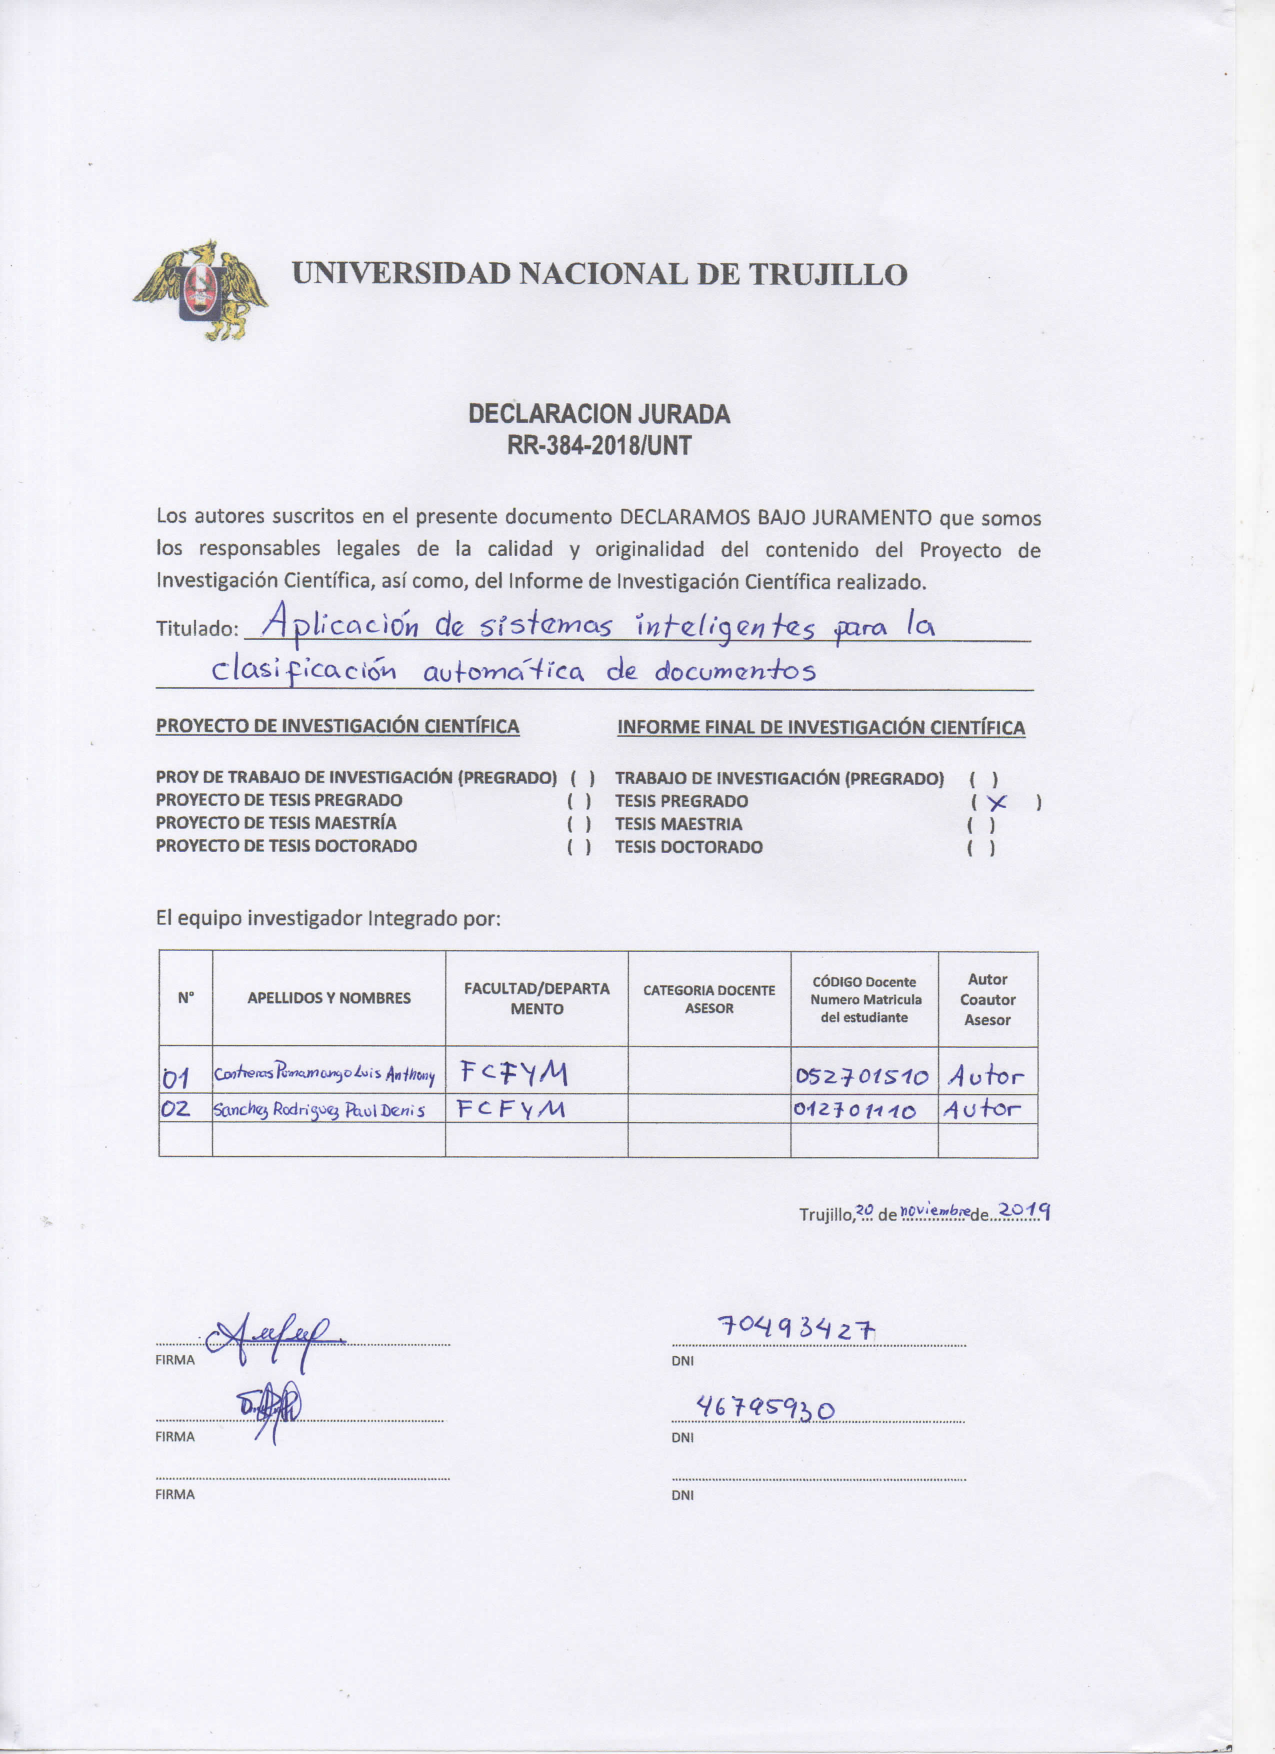
\includepdf[pages=1,pagecommand={},offset=2.7cm -2.7cm]{DECLARACION_JURADA.pdf}
%web ws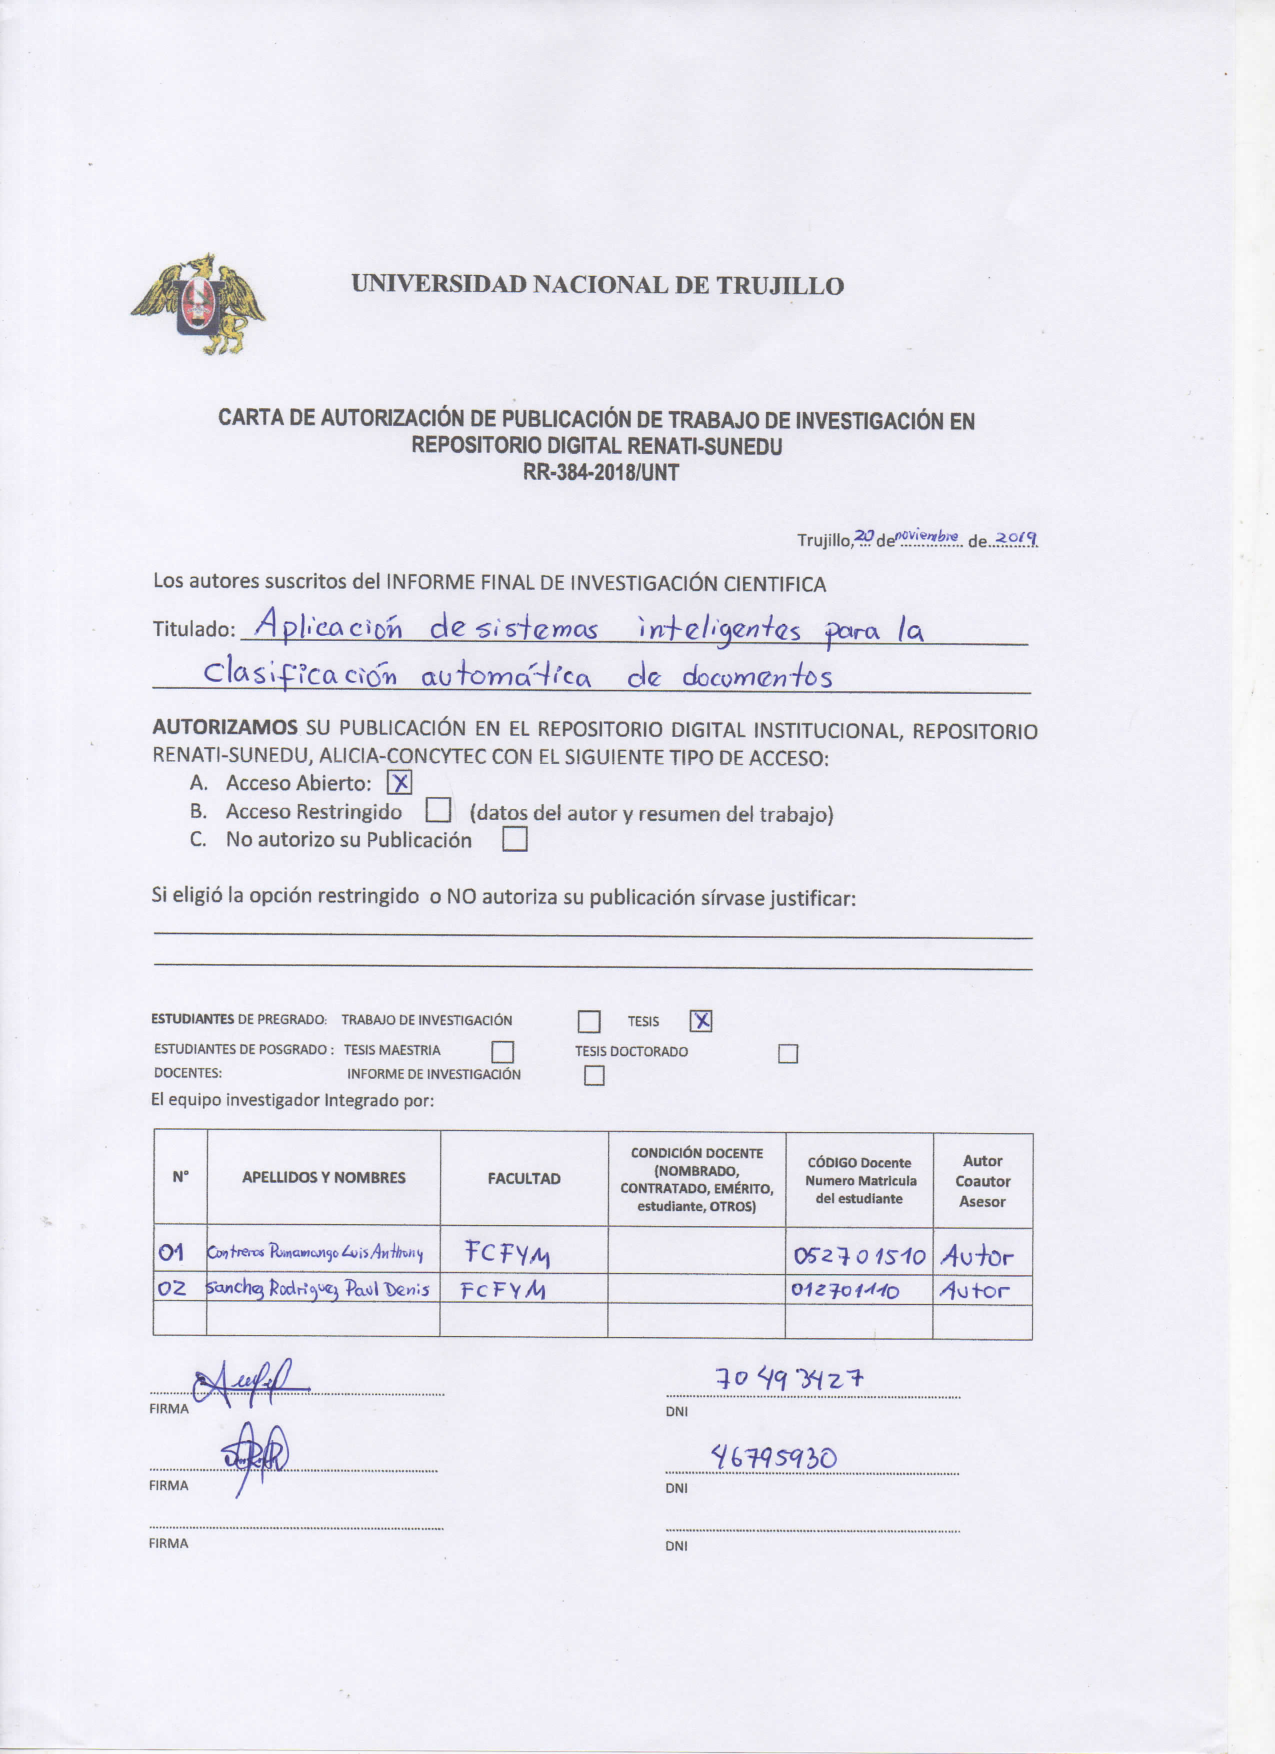
\includepdf[pages=1,pagecommand={},offset=2.7cm -2.7cm]{CARTA_AUTORIZACION.pdf}

%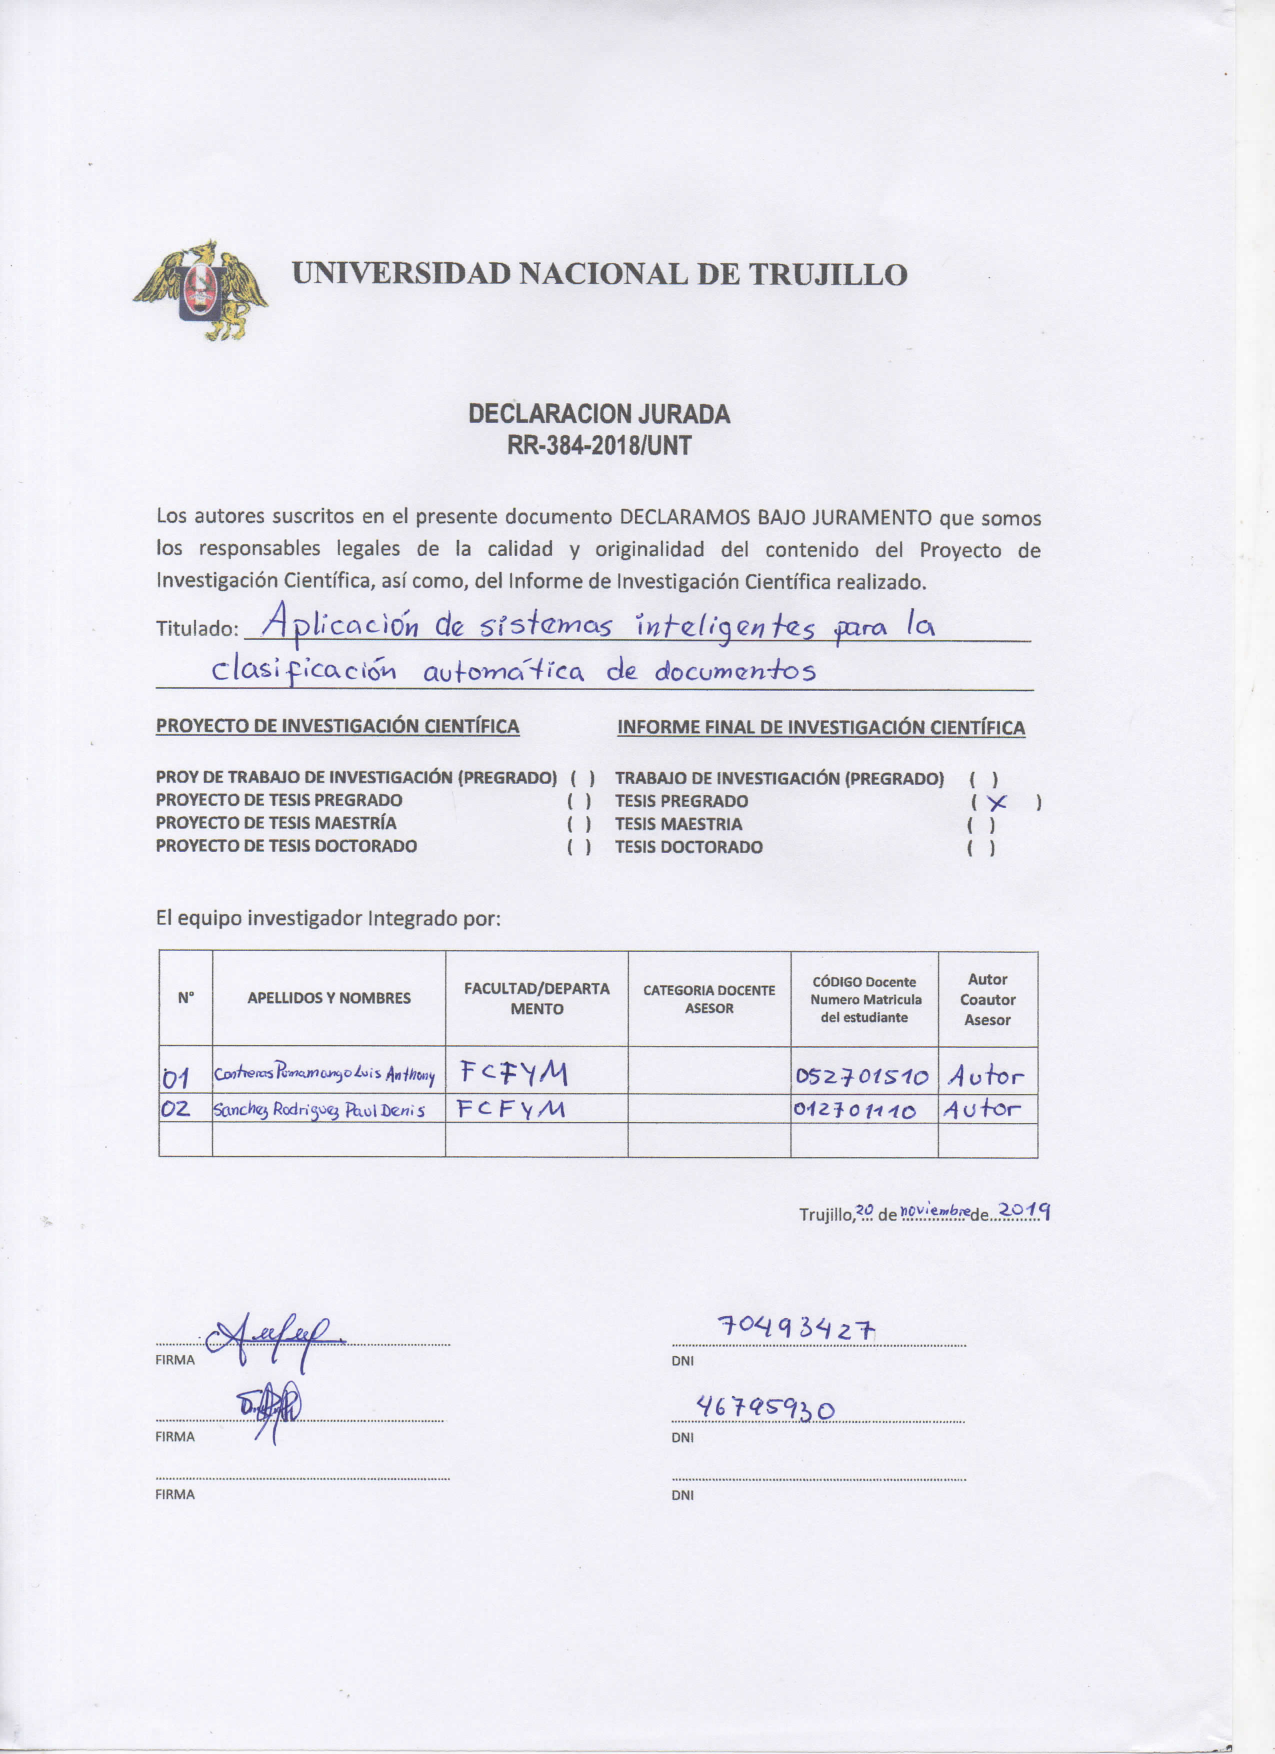
\includepdf[pagecommand={},width=\textwidth]{DECLARACION_JURADA.pdf}
%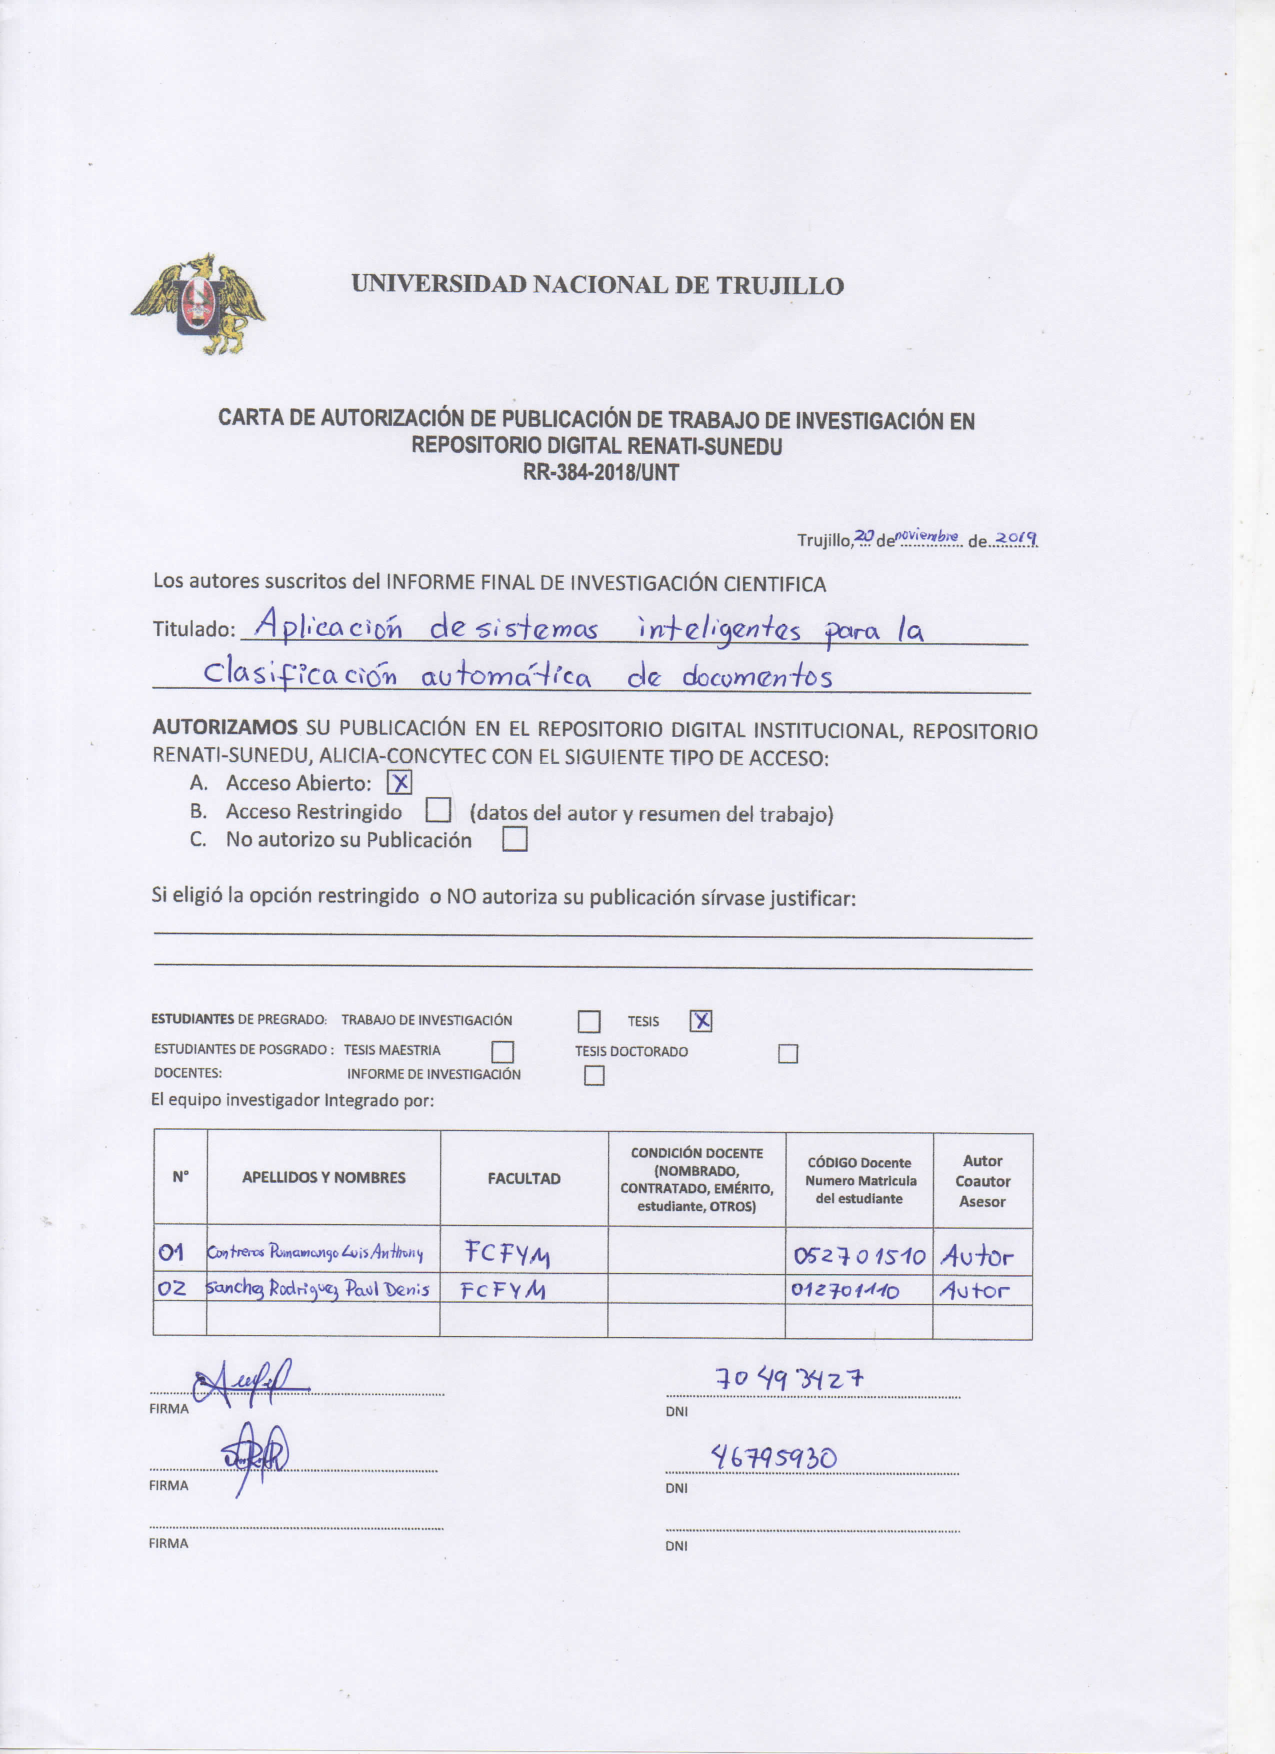
\includepdf[pagecommand={},width=\textwidth]{CARTA_AUTORIZACION.pdf}





\end{document}













